% \documentclass[conference,letterpaper,10pt]{IEEEtran}
\documentclass[conference,compsocconf,letterpaper,10pt]{IEEEtran}
\IEEEoverridecommandlockouts
\usepackage{times}
\usepackage{helvet}
\usepackage{courier}
\usepackage{listings}

%\usepackage{algorithm}
%\usepackage{algorithmicx}
\usepackage[vlined,ruled,commentsnumbered,linesnumbered]{algorithm2e}
\usepackage{algpseudocode}
\usepackage{amsmath,amsthm,amsfonts,amssymb,bm}
\usepackage{comment}
\usepackage{subfigure}
\usepackage{graphics}
\usepackage{epsfig}
\usepackage{epstopdf}
\usepackage{flushend}
\usepackage{epstopdf}

\newtheorem{theorem}{Theorem}
\newtheorem{definition}{Definition}
\newtheorem{proposition}{Proposition}
\newtheorem{lemma}{Lemma}
\newtheorem{corollary}{Corollary}

\renewcommand{\algorithmicrequire}{\textbf{Input:}} % Use Input in the format of Algorithm
\renewcommand{\algorithmicensure}{\textbf{Output:}} % Use Output in the format of Algorithm

\newcommand{\ie}{{\em i.e.}}
\newcommand{\eg}{{\em e.g.}}
\newcommand{\et}{{\em et al. }}
\newcommand{\st}{{\em s.t.}}

\renewcommand{\baselinestretch}{1}


%\title{A Strategy-Proof and Budget Feasible Online Crowdsensing Mechanism Design with \\Time-Discounting Value}
\title{\huge{A Strategy-Proof Budget Feasible Online Mechanism for Crowdsensing with Time-Discounting Values}}
\author{
Jiapeng Xie, Shuo Yang, Fan Wu,  Xiaofeng Gao, and Guihai Chen\\
Shanghai Key Laboratory of Scalable Computing and Systems\\
Shanghai Jiao Tong University, China\\
\{xjpsjtu, wnmmxy\}@sjtu.edu.cn; \{fwu, gao-xf, gchen\}@cs.sjtu.edu.cn

}

\begin{document}

\maketitle

\begin{abstract}
  %Designing an inverse game to promote interactions for intelligent participants has sparked interest within AI. We design a strategy-proof and budget feasible mechanism for an online reverse auction.
  %Budget feasible mechanism extends the classic mechanism design to the realistic setting where the total payment is bounded by a limited budget. We focus on a common online reverse auction where the provider aims to maximum the total value while the payment to the participants doesn't exceed the budget. It is much more challenging for the provider to make decisions in the online scenarios, where participants arrive dynamicly, due to short of future participants' information in contrast to offline scenarios. In this paper, we investigate online budget feasible auctions considering that the value derived from a participant decreases with time. The property of time discounting is common in intertemporal choice scenarios. But rare mechanism designs took it into account previously. We present a truthful framework in which participants will bid their true type, %although the participants will be paid differently in different time which can be menipuated by strategic participants by misreporting her information.
%instead of manipulating the market by misreporting false information.
%We also compare our design with optimal offline auction with full information, and show that our work achieves a constant competitive ratio. Our numerical results show that our design can achieve good performance in terms of total value.

Crowdsensing has become increasingly popular due to its ability to collect a massive amount of real-time data with the help of many individual smartphone users. A crowdsensing platform can utilize the collected data to extract effective information and provide services to service requesters. Due to the rationality of smartphone users, designing an incentive mechanism to compensate the participants for their resources consumption is critical in attracting more participation. Offline incentive mechanism design has been widely studied in various crowdsensing applications, whereas the online scenario, is much more challenging due to the unavailability of future information when the platform has to make user selection decisions. In this paper, we investigate the problem of online crowdsensing by considering a critical property that the values of users’ contributions decrease as time goes by. The time-discounting property is common in inter-temporal choice scenarios but has not been carefully addressed in mechanism design perspective. To handle this problem, we propose a new method to select users based on a time-related threshold, and present a strategyproof framework where participants prefer to submit their true types, instead of manipulating the market by misreporting their private information. We consider two case, one is that the total value is the summation of each participant's contributing value, the other is more general that the total value function is submodular. We name these two mechanisms TDM and TDMS. We prove that our two mechanisms can achieve computational efficiency, budget feasibility, strategy-proofness, and a constant competitive ratio. By comparing our mechanism TDM with two heuristic benchmarks, we show that our design achieves great performance in terms of the total obtained value.
\end{abstract}

\section{Introduction}

%Budget feasible mechanism design has been widely applied to many scenarios, where there is an provider wants to buy some items or services from strategic participants with a limited budget~\cite{singer2014budget}, \eg, conducting a survey with the goal of obtaining an unbiased estimator of some population statistic~\cite{roth2012conducting}, maximizing the spread of influence through a social network~\cite{kempe2003maximizing}, privacy auctions for recommender systems~\cite{dandekar2014privacy}, truthful incentives in crowdsourcing tasks~\cite{singla2013truthful} and allocating heterogeneous tasks to workers~\cite{goel2014mechanism}. %Online mechanism, which is in constrast to offline setting, has also been widely applied in many applications, \eg, electric vehicle charging~\cite{gerding2011online} and online real-time scheduling~\cite{porter2004mechanism}. This online case is much more complicated for the lack of future information when making strategies. In addition, the strategic participants may misreport their true present time for more utilities.
%Designing an online mechanism is far more complicated when making strategies due to lack of future information. In addition to cheating their true cost in the bid, strategic participants may also misreport their true present time for the purpose of earning more utilities.

%Crowdsensing is a new paradigm of applications that includes a platform and ubiquitous participants who hold mobile devices equipped with enhanced sensors~\cite{ganti2011mobile}. The platform recruits participants to upload sensing data and provide service for others. While participants will consume their own resources so they are reluctant to share their sensing capabilities. The quality and accuracy of service provided by platform is relied on the large-scale data submitted by participants, so it is required to design an incentive mechanism to incent the participants by compensating some monetary payment. Many online incentive mechnism designs have been applied in these kind of crowdsensing applications, \eg, zhao \et. designed an online incentive mechanism with budget constraint, which is modeled as an online auction~\cite{zhao2014crowdsource}, Singer and Mittal designed a pricing mechanisms for crowdsourcing markets~\cite{singer2013pricing}.

Mobile crowdsensing is a novel application paradigm that utilizes mobile devices to collect, analyze, and share their local information~\cite{ganti2011mobile,lane2010survey,Tuncay:2013:PRD:2500423.2504573,6069707,6341381}. It usually consists of a service provider, service requesters, and mobile device users. The service provider (a.k.a., the crowdsensing platform), which usually resides in the cloud, recruits participants from mobile device users to upload their sensing data, and then provides services to service requesters based on the collected information. A wide variety of applications has emerged in recent years, including NoiseTube~\cite{maisonneuve2009noisetube} and Ear-phone~\cite{rana2010ear} for noise monitoring, SignalGuru~\cite{koukoumidis2011signalguru} and CrowdAtlas~\cite{wang2013crowdatlas} for traffic monitoring, and CrowdPark~\cite{yan2011crowdpark}, Parknet~\cite{mathur2010parknet} for finding on-street parking spots.

However, a well running crowdsensing application needs massive data contributed by the participants to ensure the service quality~\cite{Wang:2015:CQO:2750858.2807513,Han:2016:PPR:2942358.2942385}. Since participating in crowdsensing tasks requires the participants to devote resource consumptions of their smartphones, participants are usually reluctant to share their sensing capabilities(\eg, \cite{Kawajiri:2014:SCI:2632048.2636064,Fan:2015:PTT:2789168.2795179,Karaliopoulos:2016:FLE:2942358.2942369}. Thus, it is necessary to design an incentive mechanism to compensate the participants. According to different settings of scenarios, two cases are often discussed, \ie, offline setting and online setting. Researches on incentive mechanism designs, such as~\cite{yang2012crowdsourcing,koutsopoulos2013optimal}, are usually based on offline scenarios, where participants are present simultaneously while the online scenarios are more common in practice, where participants arrive and leave dynamically. Designing an incentive mechanism in online scenarios is much more complicated, due to the lack of future information. Besides, it brings challenges in the realization of strategy-proofness, since participants may misreport their arrival or departure time in order to gain higher benefits. Here, intuitively, strategy-proofness means that one can maximize her benefit by truthfully revealing her private information (\eg, arrival time, departure time, or sensing cost).

%In this paper, we mainly focus on the online scenario where a provider intends to select participants to perform sensing tasks and provide them with some rewards under a limited budget. The provider then obtains the value of the sensing data and the selected participants can also receive monetary compensations after finishing sensing tasks. The key challenge for the provider is how to obtain the maximum total value and achieve incentive compatibility within the budget constraint. We model this process as a reverse auction. The bid of a participant contains her cost, value, and present time in the auction. In previous works, the value of a specific participant is often fixed, \ie, the participant has a bid of uniform value during her presence, independent of when she is selected. However, for some applications, the value of each participant's contributed data decreases with time. The time discounting property makes the problem more difficult. We aim to design an online incentive mechanism for crowdsensing with time-discounting value. The provider selects participants according to their bids (mainly their costs and time-discounting values), then gives them payments. The objective is to obtain the maximum total value and achieve strategy-proofness. It should be noted that for general utility functions, there is no truthful mechanism that can achieve a reasonable approximation ratio~\cite{singer2014budget}. In our paper, the total value of participants is simplified to the summation of values of selected participants.

We note that most existing works on online mechanism design only consider flat values, \ie, the value of each participant's contributed data is fixed during her presence. However, in many time sensitive applications (\eg, real-time traffic or noise monitoring~\cite{Chon:2014:SWP:2632048.2636066,Ji:2016:USB:2971648.2971735,Zappatore:2016:CAM:2851613.2851699,Cherian:2015:PPG:2809695.2817881}), the participants usually have time-discounting values, \ie, the value of each participant's contribution decreases as time goes by~\cite{babaioff2009secretary, wu2014strategy}. The time-discounting property really complicates the mechanism design problem. For instance, it has been proved that no online algorithm can achieve a competitive ratio better than $\Omega(\textrm{log}n/\textrm{log}\,\textrm{log}n)$ for discounted secretary problem~\cite{babaioff2009secretary}. The time-discounting property of values will bring much more difficulty, especially on the strategy-proofness. In the most of the incentive mechanisms designed for online crowdsensing, the payment to a selected participant is based on her contributation. If she can cheat her type, such as arrival time or cost, she may be selected at different time. If this time is earlier than the time with truely report information, the value of this participant calculated by the platform will be higher than the true value. For the purpose of more reward, the participant may have more incentives to bid mendaciously.

%It is known that for general utility functions, there is no truthful mechanism that can achieve a reasonable approximation ratio~\cite{singer2014budget}.

In this paper, we focus on the online scenario where a provider intends to select participants to perform sensing tasks and provide them with some rewards under a budget constraint. The objective of the problem is to maximize the total values of selected participants considering the time-discounting properties, while at the same time achieve budget feasibility and strategy-proofness. Taking the budget constraint into account brings another challenge in designing a strategy-proof mechanism, since existing budget feasible mechanism design approaches(\eg, \cite{singer2010budget, chen2011approximability,Bei:2012:BFM:2213977.2214020,Chen:2011:ABF:2133036.2133090}) are not practical in scenarios where participants' values are time-discounting.

To address these challenges, we propose a budget feasible online incentive mechanism with time-discounting values. We first consider the case where the total value is the summation of each participant's value. We define the efficiency of a participant as her value divided by her cost. Since participants arrive dynamically, we take advantage of the efficiency information of those who have arrived (we call a sample set) to calculate a threshold, and use it to guide subsequent selections. The intuition of our design is to greedily choose participants with the highest efficiencies from the sample set, and calculate their average efficiency multiplying an increasing factor as a threshold. The increasing factor is used to prevent the participants from misreporting their arrival or departure time. We divide the total time into slots. At each time slot, we select participants with efficiencies higher than the threshold within the budget constraint, and then calculate their payments. The payment scheme is carefully designed to ensure strategy-proofness and individual rationality. We prove that our mechanism can achieve a constant competitive ratio compared with the optimal solution with full information. We next consider the case where the total value is a submodular function of the selected participants, which is a more general situation. We prove that the time and cost-truthfullness can still be guaranteed by the newly designed algorithms. The numerical results show that our proposed approach has superior performance to our benchmark mechanisms.
\subsection{Key Contributions}
The main contributions of this paper is listed as follows
\begin{itemize}
\item We design an online incentive mechanism for crowdsensing. In this process, participants arrive over time. Our mechanism is designed to take advange of their efficiency to select them and give them a payment.

\item As far as we know, we are the first to consider the time-discounting property of values. To address the potential new difficulty, we design a novel algorithm to calcuate a time-related threshold to select participants and determine their payment.

\item We think about two cases according to the value function. The value function in these two cases is additive and submodular, the latter is more general.
\end{itemize}
\subsection{Paper Organization}
The rest of the paper is organized as follows. We briefly review the related work in Section II. In Section III, We introduce the model of the budget feasible online mechanism problem with time-discounting values, and recall some important solution concepts. In Section IV, we present our design of a strategy-proof online  mechanism where the value function is the summation of each participant's value. In Section V, we consider the case where the value function submodular. In Section VI, we implement and evaluate our mechanism. Finally, we conclude this paper in Section VI.
%**********************************************************
%The key challenges in a budget feasible auction are how to persue the maximum value and balance incentive compatibility and the budget constraint. It gets harder when the participants arrive dynamicly. What is noticeable is that in existing works, the value of a specific participant is often fixed, \ie, the participant has a bid of uniform value during her presence in the auction, independent of when she is selected. But in some realms, such as applications intending to collect data by crowdsensng, which are always modeled as reverse auctions, the values of participants' contributed information decrease with time. The time discounting characteristic can make the problem more difficult. In this paper, we study a type of online reverse auction, where the participants compete to provide items or services with certain time discounting values. Then the provider gives some payment to the selected participants according to their bids. The objective is to obtain  the maximum total value and achieve strategy-proofness under a limited budget. It should be noted that for general utility functions, there is no truthful mechanism achieving a reasonable approximation ratio~\cite{singer2014budget}. In our paper, the total value of participants is simplified to the summation of their values at when they are selected.
%**********************************************************
%We present a formal methonology based on the mechanism design as an inventive method in the realm of crowdsensing. which is a new paradigm of applications that includes a platform and ubiquitous participants who hold mobile devices equipped with enhanced sensors~\cite{ganti2011mobile}. The platform recruits participants to upload sensing data and then compensate them some payment according to their value. It is always modeled as a reverse auction. When designing an incentive mechanism for crowdsensing, participants' value is often taken into account when determining the task allocation and the payment. But in existing work, this value of a specific participant is often fixed, \ie, the participants have a bid of uniform value to the platform during their presences in the auction. However in many crowdsensing applications, the value of participants is time discounting, decreasing with time in majority situations. Therefore in this paper, we consider a scenario, in which participants compete for being allocated tasks and then compensated some monetary payment, but her bidding value is changing over time.  The bid of each participant is her arrival time, departure time, her cost and value to the platform which diminishes with time. The objective is to design a strategy-proof mechanism and maximize the platform's gainning value with limited budget with respect to not only the time discounting values, but also the present time and cost of the participants.

%When a participant come into this auction, she would propose a bid of her type,including her arrival and departure time indicates she will be present within these two time, a value evaluated by the paltform later and her declaring cost.  At each time slot within her present time, the mechanism will calculate a current value of her to compete with other participants for the tasks and payment. For the purpose of earning more, the participants may cheat their true type of arrival, departure time and their true cost which is her private information.
  %In our paper, when a participant come into this auction, she would propose a bid of her type,including her arrival and departure time indicates she will be present within these two time, a value evaluated by the paltform later and her declaring cost.  At each time slot within her present time, the mechanism will calculate a current value of her to compete with other participants for the tasks and payment. For the purpose of earning more, the participants may cheat their true type of arrival, departure time and their true cost which is her private information. Our objective is to design a mechanism to achieve truthfulness and maximize the total value with the constraint budget.
%The budget constraint brings a lot of tricky problems to designing a truthful mechanism. First, it is well known that we have to pay a large amount to enforce strategy-proofness, but we only have a limited budget. Second, the celebrated VCG framework is not applicable to the budget feasible online auction because the total payment will exceed the budget in some cases and computing the optimal solution is often intractable in online scenarios~\cite{Vickrey61,Clarke71,Groves73}. Moreover, existing budget feasible mechanisms are not practical since if the values of participants change with time, there will be a bias on the evaluation of values and the strategy-proofness will not be assurable any more. This motivates us to design a strategy-proof and budget feasible auction with time discounting values.

 %******************
 %In our paper, we design a new innovation for selecting participants and determining their payment. We define the efficiency of an anget as her value divided by her cost. Since participants arrive in the auction dynamicly, we consider to take advantage of the efficiency information of those participants who have arrived and proposed their bid, which is called a sample set, to calculate a threshold and use it to  guide subsequent selecting. We greedily choose participants with the highest value efficiency from the sample set and calculate a threshold similar to their average efficiency multiplying an increasing factor. This increasing factor can prevent the participants from misreporting their arrival and departure time and choosing participants with high efficiency  greedily intends to make better use of the budget. At each time slot, we use a selecting and paying scheme to select participants with efficiency higher than the threshold at that time and make sure it will not exhaust the remaining budget, then calculate the payment to them. This payment scheme can also ensure cost truthfulness and individual rationality. We prove that our mechanism can achieve a constant competitive ratio compares with the optimal auction with full information. The numerical results show that our scheme has a satisfying performance  compared with other mechanisms.
 %These two algorithms are both terminated in polynomial time, which are $O(nlogn)$ and $O(Tn^2)$ respectively.



 %Many incentive mechanisms are not approciate for this online case and existing online incentive mechanisms don't consider time discounting value of participants. In~\cite{zhao2014crowdsource} and~\cite{zhang2014free}, the authors have designed an online mechanism, but each participant is paid according to her initial proposing value and the time discounting property is not considered. We will follow their work and adjust this mechanism to achieve truthfulness with time discounting value by designing a new innovation for task allocation and payment calculation. In this paper, we present an incentive mechanism that   has a constant competitive ratio compared to optimal solution in offline setting. We assume the crowdsensing system has a deadline $T$ ,which is divided to several time slots with equal length and then we put them into several stages. At each time slot, the value of current available participants is recount by multipling a discounting factor. Then we compare this value to a threshold studied from the set of participants who has already appeared, we call it a sample set. This threshold will be calculated by an algorithm at the beginning of a stage. If the participant has an efficiency larger than this threshold, she will be selected and paid some money after finishing tasks.

%Our numerical results show that our mechanism can achieve a high performance compared to other methods.

%The rest of the paper is organized as follows. In Section 2, we briefly review related works of mechanism design. In Section 3, we introduce the model of a budget feasible online auction with time discounting values, and recall some important solution concepts used in this paper. In Section 4, we present our design of a strategy-proof online  mechanism. In Section 5, we do some simulaitons to evaluate the performance and in Section 6, we will make a conclusion.


\section{Related Works}

The problem of designing incentive mechanism for mobile crowdsensing has been extensively studied in recent years. Yang \et\cite{yang2012crowdsourcing} considered offline mechanism design problem based on stackelberg game, and proposed mechanisms for two different perspectives respectively: a user-centric model and a platform-centric model. Koutsopoulos~\cite{koutsopoulos2013optimal} designed an incentive mechanism based on a reverse auction. In his design, when the cost of a participant is received, the mechanism calculates the participant's effort level and payment vector to achieve truthfulness, and minimizes the total payment with guaranteed service quality. Later, Zhao \et\cite{zhao2014crowdsource} designed two online mechanisms, namely OMZ and OMG, that satisfied truthfulness and achieved constant competitiveness. Kumrai \et\cite{7037601} proposed a novel mechanism for participatory sensing based on the evolutionary algorithm that can maximize both the number of active participants and the sensing coverage. Singer~\cite{singer2013pricing} present a pricing mechanism for crowdsourcing. It uses a sample set to calculate the threshold, which is the lowest single price many workers may accept, with budget feasible.  Peng \et designed a quality based incentive mechanism and extend the well-known Expectation Maximization algorithm~\cite{peng2015pay}. The innovation is to apply the classical Information Theory to measure the effective contribution of sensing data. J.S.Lee \et  designed a dynamic pricing incentive mechanism based on reverse auction and focused on minimizing and stabilizing the cost while preventing participants from dropping out of sensing tasks~\cite{lee2010dynamic}.However, none of these researches took the time-discounting property into consideration.

There are few previous researches focusing on the property of time-discounting values~\cite{Frazier:2014:IE:2600057.2602897,Olariu:2014:AIA:2581555.2581569,Fujita:2014:ASA:2615731.2616036}. Babaioff \et\cite{babaioff2009secretary} studied two extensions of the secretary problem, \ie, the discounted secretary problem and weighted secretary problem. In discounted secretary problem, the benefit derived from selecting an item is its original value multiplied by a time-discounting factor. Wu \et\cite{wu2014strategy} designed a strategy-proof online mechanism with time-discounting values, and achieved a 2-competitive ratio. Unfortunately, these work cannot be easily applied to scenarios with budget constraint. 
%Singer designed a budget feasible mechanism especially when the value function is submodular~\cite{singer2010budget}. He derived an alternative characterization of the threshold payments. Chen \et designed a truthful budget feasible mechanism. It achieves a competitive ratio of less than 9, which is better than previous best known result 233.83~\cite{chen2011approximability}. Zhou \et modeled the budget-constrained bidding optimization problem as an online knapsack problem~\cite{zhou2008budget}. The threshold is calculated by a function of the fraction of capacity filled. Sarvapali and Nicholas studied the task allocation in crowdsourcing with multiple complex workflows under a budget constraint~\cite{tran2015crowdsourcing}. In~\cite{zhao2014crowdsource} and~\cite{zhang2014free}, the authors designed budget feasible online mechanisms for crowdsensing, but did not consider the time discounting property of values.

The budget feasible mechanism has been widely studied to address budget limited mechanism design problem~\cite{Zhao:2016:BOI:3001647.3001648,Balkanski:2015:MFA:2764468.2764505,Chan:2016:BFM:2936924.2936945,Goel:2014:CAB:2600057.2602851,Lee:2016:MRV:2940716.2940745,Lu:2015:IEG:2764468.2764500,Goel:2015:PCA:2799630.2757277}. Singer~\cite{singer2010budget} first designed a budget feasible mechanism for scenarios where the value function is submodular. Chen \et\cite{chen2011approximability} further proposed a truthful budget feasible mechanism. It achieves a competitive ratio of larger than $\frac{1}{9}$, which is better than previously best result 233.83. Nevertheless, these work also failed to consider the time-discounting property.
%Zhou \et\cite{zhou2008budget} modeled the budgeted bidding optimization problem as an online knapsack problem, where the threshold is calculated based on the fraction of capacity filled.

Furthermore, there are some loosely related works on online mechanism design~\cite{Naroditskiy:2013:ROM:2484920.2485023,Kesselheim:2015:SOM:2764468.2764487,Furuhata:2014:COC:2615731.2616027}, \eg,  pricing and resource allocation in cloud computing~\cite{Shi:2014:OAF:2591971.2591980}, allocating tasks with temporal constraints~\cite{nunes2015multi}, improving targeting to increase total revenue~\cite{Hummel:2015:ITI:2736277.2741079}, and dynamic resource bundling and VM provisioning in IaaS clouds~\cite{Zhang:2015:OAI:2796314.2745855}.

In contrast to the previous works, we consider both the time discounting values and the budget limitation, and propose to design a budget feasible online mechanism that can guarantee strategy-proofness with a constant competitive ratio.

%Yang \et designed an incentive mechanism using a stackelberg game and considered two different perspectives: user-centric model and platform-centric model in which each participant receives a reward proportional to her sensing time~\cite{yang2012crowdsourcing}.
%Koutsopoulos designed an incentive mechanism based on reverse auction. When receiving the cost of participants, this mechanism will calculate the participant level and payment vector to achieve truthfulness and minimize the total payment with guaranteed service quality~\cite{koutsopoulos2013optimal}. Singer~\cite{singer2013pricing} present a pricing mechanism for crowdsourcing. It uses a sample set to calculate the threshold, which is the lowest single price many workers may accept, with budget feasible.  Peng \et designed a quality based incentive mechanism and extend the well-known Expectation Maximization algorithm~\cite{peng2015pay}. The innovation is to apply the classical Information Theory to measure the effective contribution of sensing data. J.S.Lee \et  designed a dynamic pricing incentive mechanism based on reverse auction and focused on minimizing and stabilizing the cost while preventing participants from dropping out of sensing tasks~\cite{lee2010dynamic}.


\section{Preliminaries}

%In this section, we investigate a reverse auction, which is a type of auction where the roles of provider and participants are reversed. The problem is how to obtain the maximum value from the participants and guarantee the truthfulness of the market. We present the model of a budget feasible online auction with time discounting values and related solution concepts.
In this section, we present the model of our budget feasible online crowdsensing problem with time-discounting values and review some related solution concepts.
\begin{figure}[!ht]
\centering
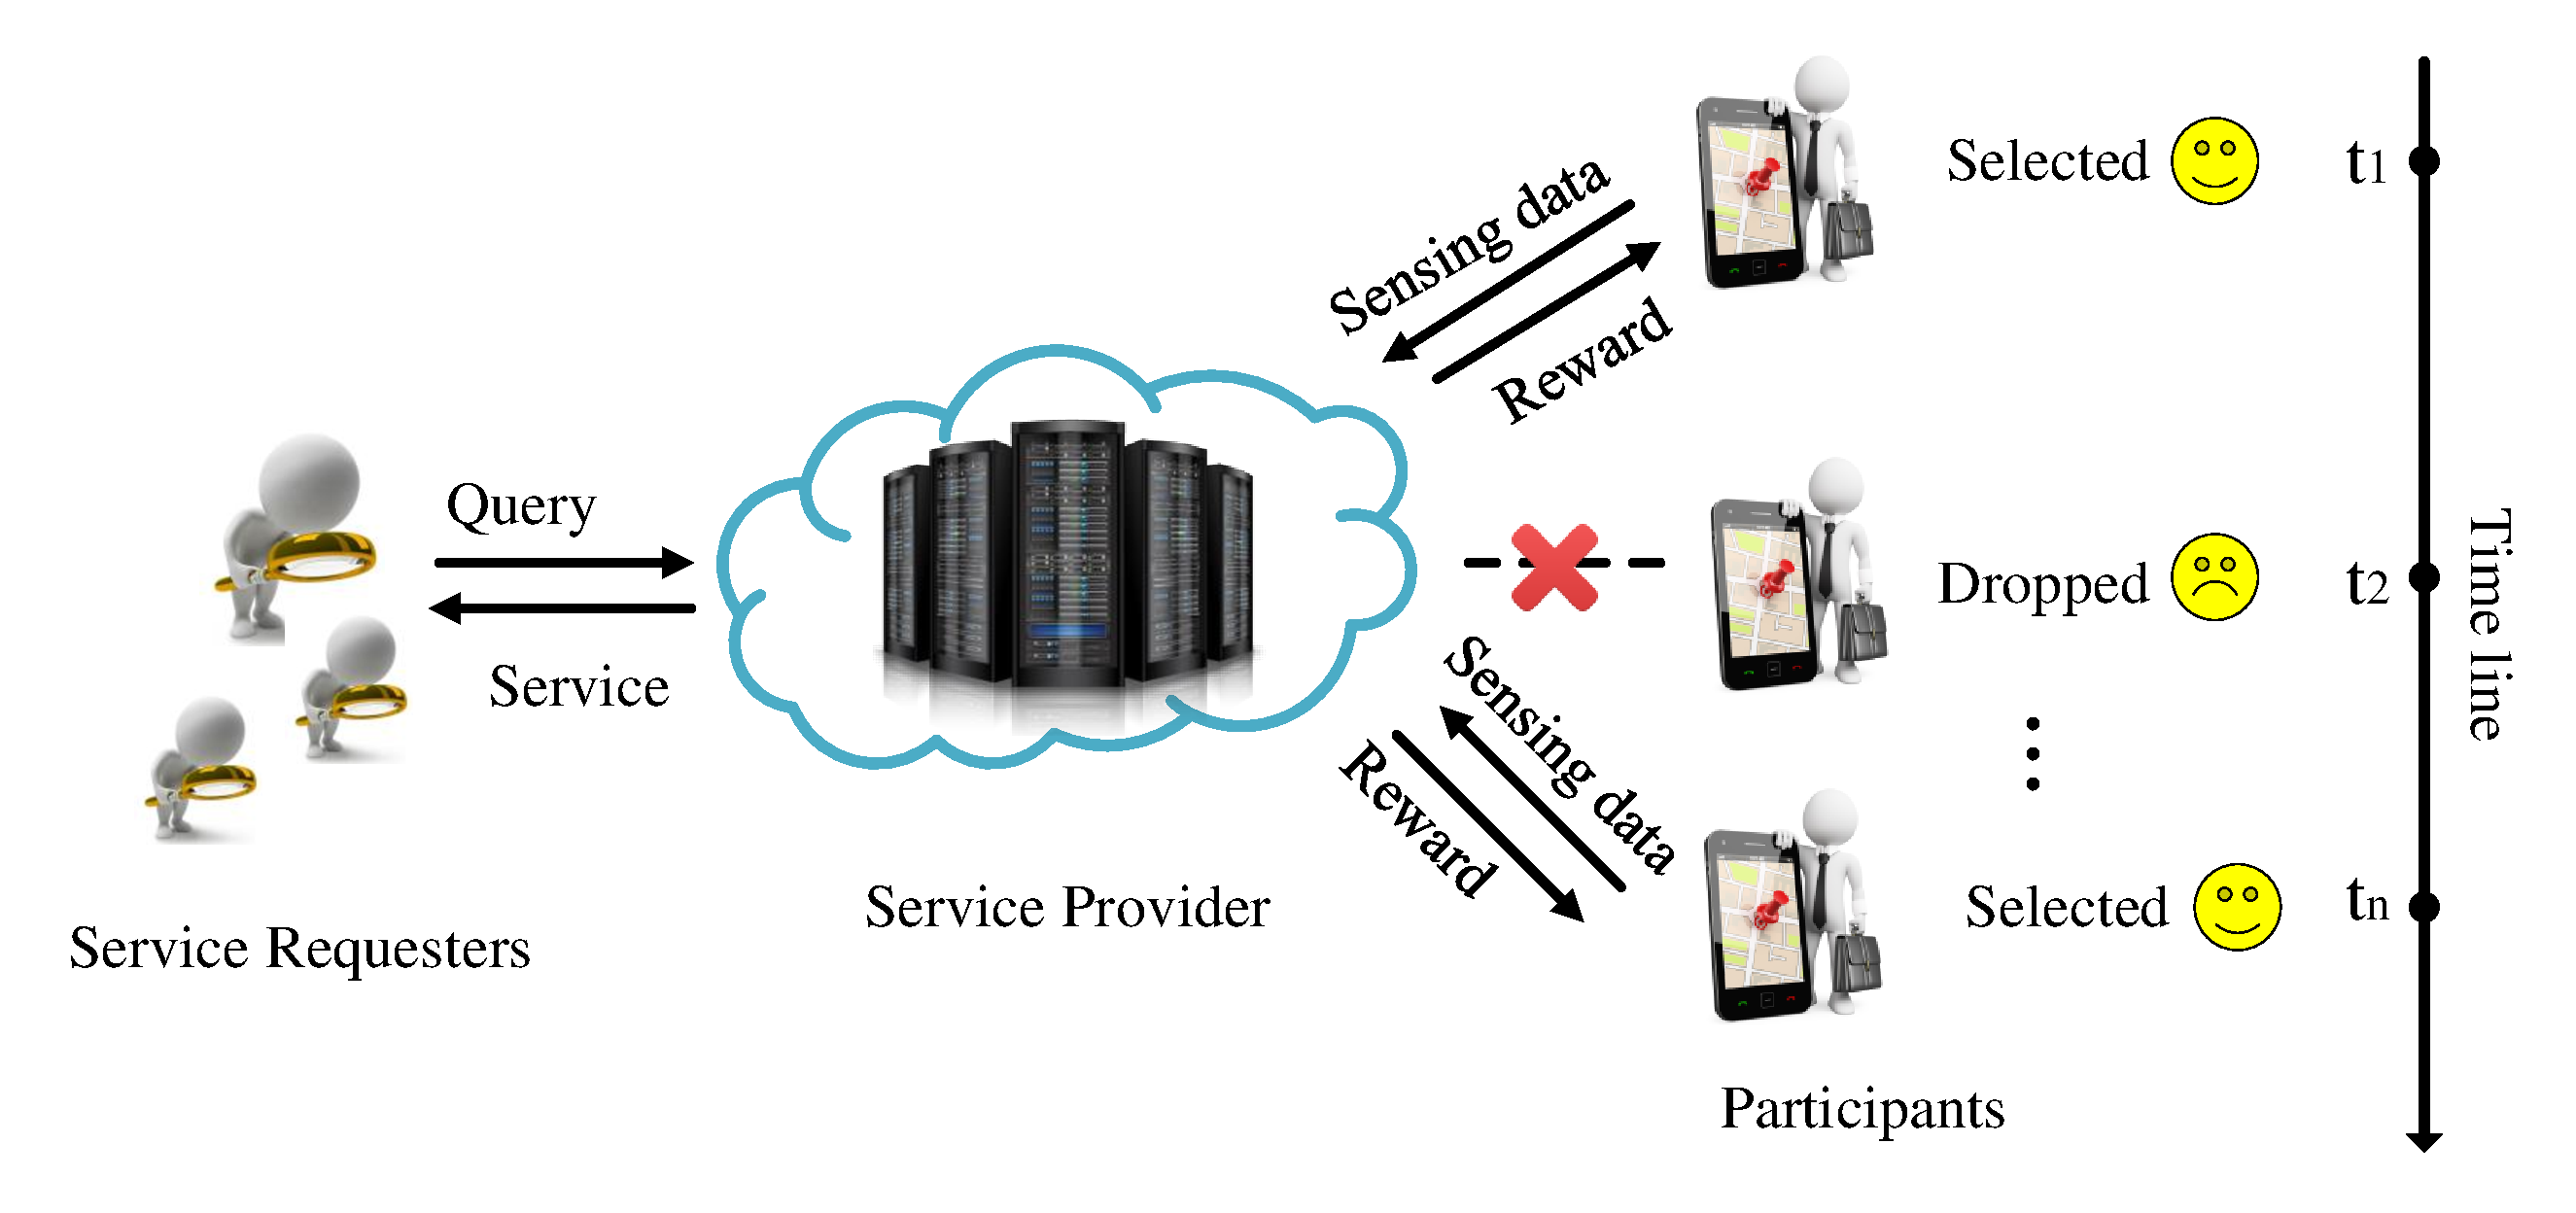
\includegraphics[width=8.5cm]{system2.pdf}
\vspace{-0.3cm}
\caption{A crowdsensing model}
\vspace{-0.5cm}
\end{figure}

\subsection{System Model}
The crowdsensing model is shown in Fig. 1. We assume that there is a service provider, some service requesters and a set of participants $\mathbb{N}=\{1,2,..., n\}.$ The provider has a limited budget $B$ to reward selected participants and intends to collect data and  provide services to service requesters. For example, the service provider collects local traffic information from participants, performs data analysis process and builds a traffic heat map, which will be used to provide real-time road congestion information to drivers.

We mainly talk about two system models, one is the case where the value function is the summeration of each participant's contributing value and the other model is more general where the value function is a submodular function. The submodular function maps a bid set or a participant set to a real positive number, \ie, the total value.

In the case where the value of a participant has nothing to do others', the total is the summeration of each participant's value. The type of each participant $i$ is $\theta_i=(a_i,d_i,v_i,c_i)$, where $a_i$ and $d_i$ represent her arrival and departure time respectively, $v_i$ denotes participant $i$'s value to the crowdsensing platform and $c_i$ represents her cost or reserve price in performing the sensing task. Here, reserve price is the minimum payment that a participant is willing to receive. In other words, each selected participant should get a payment no less than her reserve price. We note that $a_i$, $d_i$ and $c_i$ are participant $i$'s private information that are unknown to the service provider unless being reported, while $v_i$ is assumed to be $i$'s public information since participants' values can be known a prior or evaluated by the service provider \cite{peng2015pay,jin2015quality}. Upon participant $i$'s arrival, she will submit her bid $\hat{\theta}_i=(\hat{a}_i,\hat{d}_i,v_i,b_i)$ to the service provider. We note that since the participants are rational and selfish, they may cheat their arrival time, departure time, or reserve prices for the purpose of earning more payment or improving the possibility to be selected \cite{nisan2007algorithmic}, indicating that participant $i$'s bid may not be her true type. It is known that reporting earlier arrival or later departure can be prevented by heart-beat scheme~\cite{nisan2007algorithmic}, we focus on the scenario where each participant can only report an arrival time later than her true arrival time or a departure time earlier than her true departure time, \ie, $\hat{a}_i\ge a_i, \hat{d}_i\le d_i$. Participant $i$ can also misreport her reserve price $b_i \neq c_i$ to manipulate the participant selection process.

The crowdsensing process is divided into $T$ slots of equal lengths, \ie, $\mathbb{T}=\{1,2,..., T\}$. Upon a participant $i$'s arrival, the service provider will examine her bid and determine whether to select or not. Since participants arrive dynamically, the provider only knows the information of those arrived participants and has no prior knowledge of the bids of the subsequent arrivers. In the model of time-discounting values, the values of participants decrease sensitively over time. Specifically, when a participant $i$ is selected at time $t_i$, her value equals $v_i$ multiplying a discount factor. Following the settings in ~\cite{rasmussen1975choosing}, the time-discounting factor in our paper is set to $\beta^{-t}$, \ie, the value of participant $i$ at time $t_i$ is $v_i(t_i)=v_i \cdot \beta^{-t_i}$.

%The value contributed by a selected participant can also be guaranteed truthful because it's not the participant's private type. So the participant $i$ can propose a bid $\hat{\theta}_i=(\hat{a}_i,\hat{d}_i,v_i,b_i)$, $\hat{a}_i\ge a_i, \hat{d}_i\le d_i$.

We denote the set of selected participants as $\mathbb{S}$. If participant $i$ wins the auction, she will receive a payment $p_i$, having a utility of $u_i=p_i-c_i$; Otherwise, she will get zero utility, \ie,
%\begin{small}
\begin{equation}\label{equ:utilityfunction}
u_i=\left\{
\begin{aligned}
&p_i-c_i, & & i\in \mathbb{S},\\
&0, & & \text{otherwise},\\
\end{aligned}
\right.
\end{equation}
%\end{small}

In contrast to the participants who always want to maximize their own utilities, the provider expects to maximize the total obtained value $V=\sum_{i\in\mathbb{S}}v_i(t_i)$ under the budget constraint $\sum_{i\in\mathbb{S}}p_i \le B$, where $t_i$ means the time when participant $i$ is selected. The objective of our mechanism is to maximize $V$.

Similarly, in the general case where the total value function is a submodular function, each participant has a type $\theta = (a,d,p,c)$, where $a,d,c$ still represents the arrival time, departure time and her cost. Her bid is denoted as $\hat{\theta}=(\hat{a},\hat{d},p,\hat{c})$. The total value respected to a selected participant set $\mathbb{S}$ is denoted as $f(\mathbb{S})$. Our objective is to select a set $\mathbb{S}$ to maximize the function $f(\mathbb{S})$. More details are in section V.

\begin{table}[!hbp]
\caption{Notations}
\center
\begin{tabular}{cc}
\hline

Symbol & Description\\
\hline
$\mathbb{N}={1,2,...,n}$ & The participant set \\
% \hline
$B$ & The total budget\\
% \hline
$\theta_i$ & Type of participant $i$\\
% \hline
$a_i$ & arrival time of participant $i$\\
% \hline
$d_i$ & departure time of participant $i$\\
% \hline
$v_i$ & value of participant $i$\\
% \hline
$c_i$ & cost of participant $i$\\
% \hline
$\hat{\theta}_i$ & bid of participant $i$\\
% \hline
$\mathbb{T}=\{1,2,...,T\}$ & the time slot set\\
% \hline
$\beta$ & time-discounting factor\\
% \hline
$p_i$ & payment of participant $i$\\
% \hline
$\mathbb{S}$ & selected participant set\\
% \hline
$V$ & The total value\\
% \hline
$L,U$ & lower bound and upper bound of efficiency\\
% \hline
$\rho$ & efficiency threshold\\
% \hline
$V$ & The total value\\
% \hline
$\lambda$ & a system parameter\\
% \hline
$T_i$ & time stage\\
% \hline
$f$ & submodular value function\\
\hline
\end{tabular}
\\

\end{table}




\subsection{Solution Concepts}
These are several important solution concepts used in this paper from algorithmic game theory~\cite{nisan2007algorithmic}.

\begin{definition}[Dominant Strategy]
A participant $i$'s strategy $s_i$ is called her dominant strategy, if for any strategy $s'_i \ne s_i$ and any other player's strategy profile $s_{-i}$, we have $u_i(s_i,s_{-i}) \ge u_i(s'_i,s_{-i})$.
\end{definition}

\begin{definition}[Truthfulness]
An online mechanism is truthful if and only if it is the dominant strategy for every participant $i \in \mathbb{N}$ to report her true type.
\end{definition}

\begin{definition}[Individual-Rationality]
A mechanism is individual rational if and only if $u_i \ge 0$ for all participant $i \in \mathbb{N}$.
\end{definition}

\begin{definition}[Strategy-Proof\ Direct\ Revelation\ Mechanism]
A direct revelation mechanism is strategy-proof, when it satisfies both truthfulness and individual-rationality.
\end{definition}

Our objective is to design a strategy-proof and budget feasible online mechanism with time-discounting values.

\section{Mechanism Design}

In this section, we propose an online mechanism, which is named as TDM, satisfying the following properties:
\begin{itemize}
\item \textbf{Computational Efficiency}: Each step of the mechanism should be computed in polynomial time.

\item \textbf{Strategy-Proofness}: Since individual-rationality can trivially achieved, we only need to guarantee truthfulness, \ie, each participant has no incentive to misreport her type at any circumstance.

\item \textbf{Competitive Efficiency}: We define the competitive ratio as the ratio between the expected total value gained in our mechanism and the optimal value where this provider has full information of all participants~\cite{zhao2014crowdsource}. We will prove our mechanism can achieve a constant competitive ratio. In our proof, we ignore the effect of time-discounting property because it will only change the constant coefficient.
\end{itemize}

\subsection{Threshold Calculation}

In determining whether to select a participant, the service provider compares her efficiency with a threshold, which is calculated at the beginning of each stage. We will show how to define the stage in the next subsection. In this subsection, we present the algorithm to calculate the threshold, which is treated as a benchmark to guide participant selection in the current stage. Since our objective is to maximize the total value under a limited budget, a natural idea is to give higher priorities to those participants with higher efficiency for the better use of the budget. We present the procedure to calculate the threshold in Algorithm 1, which will be carried out at the beginning of each stage.

\begin{algorithm}
\BlankLine
\SetKwInOut{Input}{Input}
\SetKwInOut{Output}{Output}
\caption{GetThreshold: $GetThreshold(B, {T_k}, \mathbb{S}')$}
\label{alg:GetThreshold}
\begin{small}
\Input{Budget $B$, bid profile of sample set $\mathbb{S}'$, current stage ${T_k}$}
\Output{Threshold $\rho$}
\BlankLine
$\mathbb{D}^{T_k}\leftarrow\varnothing$;\\
  \While {$\mathbb{D}^{T_k}\neq\mathbb{S'}$}{
  	$i\leftarrow\underset{i\in\mathbb{S}'\backslash    \mathbb{D}^{T_k}}{argmax}{\frac{v_i}{b_i}}$;\\
  	\If {$b_i \le \frac{\frac{2U}{L}v_i}{\sum\limits_{j \in \mathbb{D}^{T_k}}v_j+v_i}B$}{
  		$\mathbb{D}^{T_k}=\mathbb{D}^{T_k}\cup\{i\};$
  	}
  	\lElse{
  		\textbf{break}
  	}
  }
\Return $\frac{1}{\lambda}\frac{\sum_{i\in\mathbb{D}^{T_k}}v_i}{\sum_{i\in\mathbb{D}^{T_k}}b_i}\left(\frac{U}{L}\right)^{l-k};$
\end{small}
\end{algorithm}

In the algorithm, $B$ means the capped budget in this stage, $\mathbb{S}'$ means the available sample set and $T_k$ is the beginning time of this stage. We assume each participant has a bounded efficiency between $L$ and $U$, \ie, $L \le \frac{v_i}{b_i} \le U, \forall i \in \mathbb{N}$. This procedure selects the participant with the highest efficiency into $\mathbb{D}^{T_k}$ in proper order under the constraint $b_i \le \frac{\frac{2U}{L}v_i}{\sum\limits_{j \in\mathbb{D}^{T_k}}v_j+v_i}B$. We take the average efficiency of participants in $\mathbb{D}^{T_k}$ multiplied by a stage related factor as the threshold, \ie, $\frac{1}{\lambda}\frac{\sum_{i\in\mathbb{D}^{T_k}}v_i}{\sum_{i\in\mathbb{D}^{T_k}}b_i}\left(\frac{U}{L}\right)^{l-k}$, where $\lambda$ is a system parameter and $l$ is the total number of stages.

The following results will help us to evaluate the total value of participants selected by this criterion when we estimate the competitive ratio.
\begin{lemma}
If there is a sequence of participants sorted by efficiency, \ie, 
\begin{eqnarray}
\frac{v_1}{b_1} \ge \frac{v_2}{b_2} \ge \cdots \ge \frac{v_m}{b_m} \notag
\end{eqnarray}
 and a budget $B$, then for any two participant $x$ and $y$, if $\frac{v_x}{b_x} \ge \frac{v_y}{b_y}$ and $b_y \le \frac{\frac{2U}{L}v_y}{\sum_{j<y}v_j+v_y}B$, we have
\begin{eqnarray}
b_x \le \frac{\frac{2U}{L}v_x}{\sum_{j<x}v_j+v_x}B.
\end{eqnarray}
\end{lemma}

\begin{proof}
Since $\frac{v_x}{b_x} \ge \frac{v_y}{b_y}$, it means $b_x \le \frac{v_x}{v_y}b_y$. Thus, we have:
\begin{align}
b_x&\le \frac{v_x}{v_y}b_y  \le \frac{v_x}{v_y}\frac{\frac{2U}{L}v_y}{\sum_{j<y}v_j+v_y}B\notag\\
&\le \frac{\frac{2U}{L}v_x}{\sum_{j<y}v_j+v_y}B \notag\\
&\le \frac{\frac{2U}{L}v_x}{\sum_{j<x}v_j+v_x}B\notag
\end{align}




\end{proof}
From this lemma, we can see that in Algorithm 1, if the loop is broken at some $i$, we do not need to consider another participant $j$ whose efficiency is smaller than $i$, since from $\frac{v_i}{b_i} > \frac{v_j}{b_j}$, we can infer that $b_j > \frac{\frac{2U}{L}v_j}{\sum_{l<j}v_l+v_j}B$.
\begin{theorem}Assume that there is a sequence of participants and a total budget $B$, sorted by their efficiency, \ie, $\frac{v_1}{b_1} \ge \frac{v_2}{b_2} \ge \cdots \ge \frac{v_r}{b_r}$, where the index r satisfies $\sum_{i \le r} b_r \le B$ but $\sum_{i \le r+1} b_r > B $ (changing their order number will not affect our result). Let $m$ denote the last participant satisfies $b_m \le \frac{\frac{2U}{L}v_m}{\sum_{j<m}v_j+v_m}B$. We say
\begin{small}
\begin{eqnarray}
\sum_{i=1}^{m} b_i > \sum_{i=m+1}^{r}b_i. \notag
\end{eqnarray}
\end{small}
\end{theorem}

\begin{proof}
According to lemma 1, for $i \in \{1,2,\cdots, m-1\}$, participant $i$ will also satisfy $b_i \le \frac{\frac{2U}{L}v_i}{\sum_{j<i}v_j+v_i}B$ and for $i \in \{m+1,m+2,\cdots, r\}$, participant $i$ will not satisfy this property. For the purpose of contraction, we assume that $\sum_{i=1}^{m} b_i \le \sum_{i=m+1}^{r}b_i$. Since $b_i > \frac{\frac{2U}{L}v_i}{\sum_{j<i}v_j+v_i}B$, when $i > m$,
\begin{small}
\begin{align}
\nonumber \sum_{i=m+1}^{r}b_i  &> \sum_{i=m+1}^{r}\frac{\frac{2U}{L}v_i}{\sum_{j<i}v_j+v_i}B \\
\nonumber &> \sum_{i=m+1}^{r}\frac{\frac{2U}{L}v_i}{\sum_{j=1}^{m}Ub_j+\sum_{j=m+1}^{i}Ub_j}B \\
\nonumber &> \sum_{i=m+1}^{r}\frac{\frac{2U}{L}v_i}{\sum_{j=m+1}^{r}Ub_j+\sum_{j=m+1}^{r}Ub_j}B \\
\nonumber &> \sum_{i=m+1}^{r}\frac{\frac{2U}{L} \cdot L \cdot b_i}{\sum_{j=m+1}^{r}Ub_j+\sum_{j=m+1}^{r}Ub_j}B = B .
\end{align}
\end{small}
We have a contradiction.
\end{proof}

\begin{corollary}
Using the same notation in Theorem 1, we say
\begin{equation}
\sum_{i=1}^{m} v_i > \frac{L}{U+L}\sum_{i=1}^{r} v_i. \notag
\end{equation}
\end{corollary}

%\begin{proof}Since  $\sum_{i=1}^{m} b_i > \sum_{i=m+1}^{r}b_i$, then $\sum_{i=m+1}^{r} v_i \le U\sum_{i=m+1}^{r} b_i \le U\sum_{i=1}^{m} b_i \le \frac{U}{L}\sum_{i=1}^{m} v_i$. So $\sum_{i=1}^{r} v_i = \sum_{i=1}^{m} v_i + \sum_{i=m+1}^{r} v_i \le (1+\frac{U}{L})\sum_{i=1}^{m} v_i$, \ie, $\sum_{i=1}^{m} v_i > \frac{L}{U+L}\sum_{i=1}^{r} v_i$.
%\end{proof}

\begin{proof}
Since  $\sum_{i=1}^{m} b_i > \sum_{i=m+1}^{r}b_i$, then
\begin{align}
\nonumber \sum_{i=m+1}^{r} v_i &\le U\sum_{i=m+1}^{r} b_i  \le U\sum_{i=1}^{m} b_i \le \frac{U}{L}\sum_{i=1}^{m} v_i.
\end{align}
So $\sum_{i=1}^{r} v_i = \sum_{i=1}^{m} v_i + \sum_{i=m+1}^{r} v_i \le (1+\frac{U}{L})\sum_{i=1}^{m} v_i$, \ie, $\sum_{i=1}^{m} v_i > \frac{L}{U+L}\sum_{i=1}^{r} v_i$.
\end{proof}

\subsection{Participant Selection and Payment Determination}
Having presented a method to calculate the threshold, we now use it to guide participant selection in this subsection. First, we compute the $2^i$ quantile, given the distribution of the arrival time of participants~\cite{singer2013pricing}. We denote $T_k$ as the moment before which participants arrive with the probability $2^{-k}$. Then, we get a set $\{T_1, \dots,T_l\}$.  Based on this set, we divide the time slots into several stages, where each stage begins at $T_i$ and ends at $T_{i-1}$. At each $T_i$, we calculate the threshold to guide the participant selection in this stage. We present our algorithm in Algorithm 2 to elaborate the processes of participant selection and payment calculation.
%$T_{i+1} = \lfloor T_i\rfloor$ and let $T_l = 1$

\begin{algorithm}
\BlankLine
\SetKwInOut{Input}{Input}
\SetKwInOut{Output}{Output}
\caption{Participant Selection$\&$Payment Calculation}
\label{alg:participant selection}
\begin{small}
\Input{Budget $B$, set $\{T_1, \dots,T_l\}$}
$t\leftarrow1, \rho\leftarrow\varepsilon, , x\leftarrow l$;\\
$B^{'} \gets \frac{1}{2^{l}}B, \mathbb{S}\leftarrow\varnothing, \mathbb{S}'\leftarrow\varnothing, \mathbb{A}\leftarrow\varnothing$;\\
  \For{$t=1$ to $T$}{
  	\If{some participant $i$ arrives}{
  		$\mathbb{A}\leftarrow\mathbb{A}\cup\{i\}$;
  	}
  	\ForEach{participant $i$ in $\mathbb{A}$}{
  		\If{$\frac{v_i(t)}{b_i} \ge \rho$ and $\frac{v_i(t)}{\rho} \le B'-\sum_{j\in\mathbb{S} }p_j$}{
  			$p_i\leftarrow\frac{v_i(t)}{\rho}$;\\
  			$\mathbb{S}\leftarrow\mathbb{S}\cup \{i\}$;
  		}
  	}
  	$\mathbb{A}\leftarrow\mathbb{A}\backslash\mathbb{S}$;\\
  	Remove all participants that depart in $t$ from $\mathbb{A}$ and add them to $\mathbb{S}'$; \\
  	\If{$t=T_x$}{
  		$\rho\leftarrow$$GetThreshold(B', T_x, \mathbb{S}')$;\\
  		$x\leftarrow{x-1}, B'\leftarrow 2B'$;
  	}
  }
\end{small}
\end{algorithm}

The algorithm iterates from $t=1$ to $t=T$. At each time $t$, it adds all newly arrived participants to $\mathbb{A}$ , where $\mathbb{A}$ represents the participants who have arrived and not been selected or left the auction. If participant $i$ has an efficiency  $\frac{v_i(t)}{b_i} \ge \rho$ at that time and $\frac{v_i(t)}{\rho} \le B'-\sum_{j \in\mathbb{S}}p_j$, she will win the auction and be compensated with payment $p_i$ corresponding to her value at that time. Otherwise, she will be dropped and wait to be selected next time until her departure time.

If a participant has won the auction at some time, she will not be considered later on. For the purpose of truthfulness, we remove all departed participants from $\mathbb{A}$ and add them to $\mathbb{S}'$ which is the sample set. At the beginning of next stage $T_i$, the threshold and the remaining budget will be updated.

\subsection{Mechanism Analysis}

In this subsection, we analyze our proposed mechanism.

\begin{theorem}
The mechanism is computationally efficient.
\end{theorem}

\begin{proof}
In each time slot $t$, for each participant who arrives at this time, it takes up to $O(n)$ to decide whether to select her. So the total time cost in each time slot is bounded by $O(n^2)$. It costs at most $O(nlogn)$ to calculate the threshold. Thus, the time complexity of this mechanism is $O(Tn^2)$.
\end{proof}

\begin{theorem}
The mechanism is budget feasible.
\end{theorem}

\begin{proof}
Since the total payment of each stage never exhaust the allocated budget, we can see that the total payment will not exceed the total budget.
\end{proof}

\begin{theorem}
The mechanism is time-truthful.
\end{theorem}

\begin{proof}
A mechanism is time-truthful if participants cannot
obtain higher utilities by simply misreporting their arrival or departure time~\cite{zhao2014crowdsource}. We prove that for participant $i$, proposing her true arrival and departure time is a dominant strategy. Recall that each participant has a type $(a_i,d_i,v_i,c_i)$ and a bid $(\hat{a}_i,\hat{d}_i, v_i,b_i)$, $\hat{a}_i\ge a_i, \hat{d}_i\le d_i$. We fix the bids of all but participant $i$. If she proposes her true type, we consider two cases.

\textbf{Case 1}: She can win the auction  at time $t$ which belongs to  stage $[T_a,T_{a-1}]$. If $\hat{a}_i<t$, since she cannot win the auction until $t$, she won't be paid more. If $\hat{a}_i>t$, we assume she will win the auction at time $\hat{t}$ which belongs to the stage $[T_b,T_{b-1}]$. Let $\rho_a$ and $\rho_b$ be the threshold of these two stages respectively, \ie, $\rho_a=GetThreshold(B_a,T_a,\mathbb{S}_a)$ and $\rho_b=GetThreshold(B_b,T_b,\mathbb{S}_b)$. The set $\mathbb{D}$ in $Algorithm\ 1$ is denoted as $\mathbb{D}^{T_a}$ and $\mathbb{D}^{T_b}$ respectively. So $\rho_a =\frac{1}{\lambda}\frac{\sum_{i\in\mathbb{D}^{T_a}}v_i}{\sum_{i\in\mathbb{D}^{T_a}}b_i}\left(\frac{U}{L}\right)^{l-a}$ and $\rho_b =\frac{1}{\lambda}\frac{\sum_{i\in\mathbb{D}^{T_b}}v_i}{\sum_{i\in\mathbb{D}^{T_b}}b_i}\left(\frac{U}{L}\right)^{l-b}$. The payments calculated in these two time slots are $p_a=\frac{v_i(t)}{\rho_a}$ and $p_b=\frac{v_i(\hat{t})}{\rho_b}$ respectively. So we have
%\begin{small}
\begin{equation}
\frac{p_a}{p_b}=\frac{v_i(t)}{v_i(\hat{t})}\frac{\rho_b}{\rho_a}=\frac{v_i \cdot \beta^{-t}}{v_i \cdot \beta^{-\hat{t}}}\frac{\frac{1}{\lambda}\frac{\sum_{i\in\mathbb{D}^{T_b}}v_i}{\sum_{i\in\mathbb{D}^{T_b}}b_i}\left(\frac{U}{L}\right)^{l-b}}{\frac{1}{\lambda}\frac{\sum_{i\in\mathbb{D}^{T_a}}v_i}{\sum_{i\in\mathbb{D}^{T_a}}b_i}\left(\frac{U}{L}\right)^{l-a}}.
\end{equation}
%\end{small}
We assume that every participant has a bounded efficiency, \ie, $L \le \frac{v_i}{b_i} \le U$, then we have
\begin{equation}
\frac{p_a}{p_b} \ge \beta^{(\hat{t}-t)} \frac{L}{U}  \cdot \left(\frac{U}{L}\right)^{a-b} > 1.
\end{equation}

The above inequality is satisfied because if $T_a=T_b$, then $\rho_a=\rho_b$. It can be seen that $p_a \ge p_b$, since the time-discounting value reduces her payment. If $T_a < T_b$, the inequality is satisfied as well. This indicates that the participant will get a lower payment and she will have no incentive to cheat her arrival time. The analysis on the departure time is similar.

\textbf{Case 2}: If this participant can not win this auction, she will not satisfy the condition at any time within her present time. She has no incentive to misreport her arrival or departure time since she won't get more payment.
\end{proof}

\begin{theorem}
The mechanism is cost-truthful.
\end{theorem}

\begin{proof}
A mechanism is cost-truthful if participants cannot obtain higher utilities by simply misreporting their reserve prices~\cite{zhao2014crowdsource}. Different from previous works on the truthfulness problem which claim that an online auction is cost-truthful only if it is bid-independent, the case in our mechanism is more complicated because of the time discounting property. We consider the following two cases.

\textbf{Case 1}: Participant $i$ can win the auction at time slot $t_a$ which is in the stage $[T_a,T_{a-1}]$. If she declares a smaller bid $b_i$ and wins the auction earlier, say at time $t_b$, which is in stage $[T_b,T_{b-1}]$, it would be impossible. We note that if some participant wins at $t_a$, she cannot win the auction before that time. We notice that in time slot $t_a$, $\frac{v_i(t_a)}{c_i} \ge \rho_a$, so according to the proof in Theorem $4$, $\frac{v_i(t_b)}{c_i} \ge \rho_b$ still holds. But she was not allocated at that time $t_b$, the only reason is that her payment exceeds the remaining budget. So this participant will not gain more payment at $t_b$ as well. Obviously, declaring a larger bid won't help her gain more.

\textbf{Case 2}: Participant $i$ loses this auction. This means at any time $t$, $\frac{v_i(t)}{c_i} \le \rho$, or $\frac{v_i(t)}{c_i} \ge \rho$ but $\frac{v_i(t)}{\rho} \ge B'-\sum_{j \in\mathbb{S}}p_j$. The second condition means at that time, the payment calculated in our algorithm will exhaust the remaining budget. No matter how the participant changes her bid, this  block always exists. If she declares a larger bid, the inequations still hold. If she declares a smaller bid $b_i$ and gets a payment $\frac{v_i(t)}{\rho}$. Since $\frac{v_i(t)}{c_i} \le \rho$, this new payment will be less than her true cost $c_i$ and her utility will be less than zero. A strategic participant has no incentive to misreport in this case.
\end{proof}

\begin{theorem}
The mechanism is time-truthful and cost-truthful.
\end{theorem}
\begin{proof}
We prove that participants cannot obtain higher utilities by simultaneously misreporting their arrival or departure time and their reserve prices. We consider the case that a participant may misreport her present time and cost at the same time. It should be noted that the payment has no $direct$ relationship with the bid $b_i$. If this participant can win the auction at $t$ and she can be selected after time $t$ by misreporting her present time, as we show in Theorem $4$, the payment decreases. If she can be selected at a time before $t$, it is equivalent to the case in Theorem $5$. If the participant can't win the auction at any time, she has no incentive to misreport her bid $b_i$ within the present time $[a_i, d_i]$.
\end{proof}

The above theorems indicate the truthfulness of our mechanism. To quantify the performance of the mechanism, we compare the total value with the optimum.

\begin{theorem}
The mechanism has a constant competitive ratio. In a large-scale crowdsensing system, this competitive ratio approaches to $\left(\frac{U}{L}\right)^{2-2l}\frac{U}{16(U+L)}(1-\frac{1}{e})$.
\end{theorem}
\begin{proof}
Here, a large-scale crowdsensing system means that there are a large number of participants and a single participant cannot affect the market significantly~\cite{6979011}. Let $\mathbb{S}'$ be the sample set at time $T_1$ and run the $GetThreshold$ procedure on this set, we get a threshold $\rho$. Khuller \et\cite{khuller1999budgeted} proposed a \emph{modified greedy algorithm}, which has a constant competitive ratio $\frac{1}{2}(1-\frac{1}{e})$. 

\begin{algorithm}
\BlankLine
\SetKwInOut{Input}{Input}
\SetKwInOut{Output}{Output}
\caption{Modified greedy algorithm}
\label{alg:greedy}
\begin{small}
\Input{Budget $B$, the participant set $\mathbb{P}=\{p_1,p_2,...,p_n\}$}
\Output{Selected Participants}
\BlankLine
$\mathbb{S}\rightarrow\emptyset,C\rightarrow 0,\mathbb{U}\rightarrow\mathbb{S}$;\\
\While{$\mathbb{U}\neq\emptyset$}{
	select $p_i \in mathbb{U}$ that maximizes $\frac{v_i}{c_i}$;\\
	\If{$C+c_i\le B$}{
		$\mathbb{S}\rightarrow\mathbb{S}\cup{p_i}$;\\
		$C\rightarrow C+c_i$;\\
	}
	$\mathbb{U}\rightarrow\mathbb{U}\backslash\{p_i\}$;
}
Select a participant $p*$ that maximizes $v*$ over $\mathbb{P}$;\\
If $V(\mathbb{S})\ge v*$, output $\mathbb{S}$, otherwise, output $\{p*\}$;
\end{small}
\end{algorithm}




We assume the output of this algorithm on $\mathbb{S}'$ is ${v_1,v_2,\cdots, v_r}$ and $\sum_{i \le r} b_r \le B'$ but $\sum_{i \le r+1} b_r > B' $. $B'$ equals $\frac{B}{2}$ here. In the last step in \emph{modified greedy algorithm}, we choose the participant with the highest value or those selected by the  well-known greedy strategy. But when the number of participants are very large, the output will have a high probability to be the latter. So the expected output of this algorithm approaches to the greedy output when $n$ is large enough. Our analysis is based on this fact that the bid of each participant is extremely tiny compared with the total budget. Assume that a bid satisfies $b_i \le \epsilon B$. So $\sum_{i \le r} b_i \ge B'-b_{r+1} \ge B'-\epsilon B =(\frac{1}{2}-\epsilon)B$. Let $\mathbb{S}_{OPT}$ be the optimal set when the provider has full information of the participants, $\mathbb{S}^1$ be the set of participants who arrive and departure before time $T_1$ in $\mathbb{S}_{OPT}$, and $\mathbb{S}^2$ be the set of participants who arrive and departure in the last stage in $\mathbb{S}_{OPT}$. When participants arrive uniformly (this assumption will only affect the constant coefficient), it is easy to show the expected value in this set is $E[V(\mathbb{S}^1)]=\frac{1}{4}E[V(\mathbb{S}_{OPT})]$. So the ratio of \emph{modified greedy algorithm} to the optimal solution $\mathbb{S}_{OPT}$ is at least a constant.

Now, we compare the value of the participants selected in the last stage by our mechanism with the value of those selected by the \emph{modified greedy algorithm}. If this ratio is a constant, the competitive ratio of our algorithm will be a constant.

We consider the participants who fail to be selected. We set the parameter $\lambda$ to satisfy this condition: $\frac{\left(\frac{U}{L}\right)^{l-1}}{\lambda} \le \frac{1}{2}$. Then we claim that with a high probability, there will be at least one participant has an efficiency larger than $\rho$, \ie, $\frac{v_i(t_i)}{b_i} \ge \rho$ but $\frac{v_i(t_i)}{\rho }+\sum_{j}p_j > B$. The threshold in this stage is $\rho$, which is smaller than $\frac{U}{2}$ with a selection of the parameter $\lambda$. Denote $P_i$ as the probability of the participant $i$ having an efficiency higher than $\rho$. So for any number $k$ of participants, there will be at least one participant having the efficiency larger than $\rho$ with a probability $P=1-\prod_{i=1}^kP_i$, which tends to be 1 when $k$ is large. Based on this, our expected total value approaches to the total value estimated below. For this participant $i$:
\begin{small}
\begin{align}
\nonumber &v_i(t_i) \ge (B-\sum_{j}p_j)\rho \\
\nonumber \Rightarrow\ &v_i \ge (B-\sum_{j}p_j)\rho
\end{align}
\end{small}

Since $v_i \le Ub_i \le U\epsilon B$, we have $(B-\sum_j{p_j})\rho \le U\epsilon B$, \ie, $\sum_j{p_j} \ge (1-\frac{U\epsilon}{\rho})B$. If we can choose an appropriate parameter $\lambda$  \st  $1-\frac{U\epsilon}{\rho} > 0$ , the total payment will be at least a constant fraction of the total budget $B$. Then, we have:
\begin{small}
\begin{align}
\nonumber \sum_{i \in\mathbb{S}} v_i &\ge \sum_{i \in\mathbb{S}}\rho_{i} \cdot p_i \\
\nonumber &\ge \sum_{i \in\mathbb{S}}\left(\frac{U}{L}\right)^{-l}\rho \cdot p_i\\
&\ge \frac{v_1+\dots+v_m}{\lambda B}\left(\frac{U}{L}\right)^{1-l}\sum_{i \in\mathbb{S}}p_i,
\end{align}
\end{small}
where $\rho_i$ denotes the threshold when participant $i$ is selected. We can get
\begin{eqnarray}
\frac{\sum_{i \in\mathbb{S}}v_i}{v_1+\dots+v_m} > \frac{ (1-\frac{U\epsilon}{\rho})}{\lambda}\left(\frac{U}{L}\right)^{1-l}
\end{eqnarray}

The requirement for $\lambda$ is:
\begin{align}
 \nonumber U\epsilon < \frac{\frac{v_1+\dots+v_m}{b_1+\dots+b_m}\left(\frac{U}{L}\right)^{l-1}}{\lambda}, 
 \end{align}
 \ie, $ \lambda < \frac{\frac{v_1+\dots+v_m}{b_1+\dots+b_m}\left(\frac{U}{L}\right)^{l-1}}{U\epsilon}. $  It's noticed that $\frac{v_1+\dots+v_m}{b_1+\dots+b_m} \ge L$, so we can relax our restricted condition to $ \lambda < \frac{L\left(\frac{U}{L}\right)^{l-1}}{U\epsilon}$, \ie, $\lambda \le \frac{\left(\frac{U}{L}\right)^{l-2}}{\epsilon}.$

Based on the analysis above and the $Corollary$ 1, the expected competitive ratio is at least
\begin{small}
\begin{eqnarray}
\small
P\frac{L}{8(U+L)}(1-\frac{1}{e})\frac{ (1-\frac{U\epsilon}{\rho })}{\lambda}\left(\frac{U}{L}\right)^{1-l}.
\end{eqnarray}
\end{small}

We note that although $\rho$ is a variable, it is bounded because of the bounded efficiency. So we can take the lower bound to be the competitive ratio. The calculation process is omitted here. When $\epsilon$ and $P$ approach to 0 and 1 respectively, the competitive ratio is:
\begin{eqnarray}
\frac{L}{8\lambda(U+L)}(1-\frac{1}{e})\left(\frac{U}{L}\right)^{1-l}.
\end{eqnarray}

The restriction condition on the parameter $\lambda$ is:
\begin{align}
2\left(\frac{U}{L}\right)^{l-1}\le\lambda < \frac{1}{\epsilon}\left(\frac{U}{L}\right)^{l-2}.
\end{align}

When $\epsilon$ is sufficiently small, we can always find such a parameter $\lambda$ equals $2\left(\frac{U}{L}\right)^{l-1}$. Then the expected competitive ratio is:
\begin{align}
\left(\frac{U}{L}\right)^{2-2l}\frac{U}{16(U+L)}(1-\frac{1}{e}). 
\end{align}
\end{proof}
% Due to limitations of space, we omit the proof here.
%\begin{equation}
%\left\{
%\begin{aligned}
%\frac{\left(\frac{U}{L}\right)^{l-1}}{\lambda}<\frac{1}{2}\\
%\lambda < \frac{\left(\frac{U}{L}\right)^{l-2}}{\epsilon}\\
%\end{aligned}
%\right.
%\end{equation}
\section{Mechanism with Monotone Submodular Value Function}
In this section, we propose an online mechanism, which is named as TDMS, for the general model.
\subsection{System Model}
The general model is similar with the model we have presented in section III. However the task is divided into some sub-tasks and the bid of each participant includes the set of sub-tasks she can finish. The bid of of participant $i$ is $\theta_i=(a_i,d_i,p_i,c_i)$, where we use the same notation $p_i$ to represent the sub-task set of participant $p_i$ for brevity.
\subsection{Mechanism Design}
In last section, we propose an incentive mechanism for online crowdsensing with time-discounting values, specifically the total obtained value is linear summeration of value contributed by each participant, \ie,
%\begin{small}
\begin{equation}
V=\sum\limits_{i \in \mathbb{S}}v_i(t_i)
\end{equation}
%\end{small}
However in many scenarios~\cite{zhao2014crowdsource}, the value of participants to the platform is $f(\mathbb{S})$, where $f$ is a monotone submodular function ans $\mathbb{S}$ is the selected participants set. Particularly, we have solved the case where the value function $f(\mathbb{S})=\sum\limits_{i \in \mathbb{S}}v_i(t_i)$. Here we give the definition of monotone submodular function.
\begin{definition}[Monotone Submodular Function]
A function $f:2^{[n]}\to \mathbb{R}$ is submodular if and only if:
\begin{equation}
f(\mathbb{A}\cup\{i\})-f(\mathbb{A})\ge f(\mathbb{B}\cup \{i\})-f(\mathbb{B}). \forall \mathbb{A}\subseteq\mathbb{B} \notag
\end{equation}
\end{definition}
In existing works focused on submodular function maximation in the realm of incentive mechanism design for crowdsensing, the marginal value contributed by a participant is related to the order she is selected. Besides, the total value is only decided by the tasks of the selected participants. However in this paper, considering the time-discounting property, the value function is a bit more complicated. We still use the notation $f$ to denote the value function without considering time-discounting value. When a participant $i$ is selected at time $t_i$, her marginal contribution given a subset $\mathbb{S}$ is $f_{i|\mathbb{S}}=(f(\mathbb{S}\cup\{i\})-f(\mathbb{S}))\times\beta ^{-t_i}$.
Assume the selected participant set is $\{i_1,i_2,...,i_n\}$ and their selected time is $t_{i_1},t_{i_2},...,t_{i_n}$ respectively. So when select the first participant $i_1$, her real contribution value is $f_{t_{i_1}}(\{i_1\})=f(\{i_1\})\times \beta^{-t_{i_1}}$. The value contributed by the secondly selected participant without consider time-discounting property is $f(\{i_1,i_2\})-f(\{i_1\})$ and her true contribution should be discounted by timing $\beta^{t_{i_2}}$. Thus, the total value contributed these two participants is $f_{t_{i_1},t_{i_2}}(\{i_1,i_2\}) = f_{t_{i_1}}(\{i_1\})\times \beta^{-t_{i_1}} + [f(\{i_1,i_2\})-f(\{i_1\})]\times\beta^{-t_{i_1}}$. We use $\tilde{f}$ to substitute $f$ when considering time-discounting property. So, the total value contributed by all these $n$ participants are
\begin{align}
&\tilde{f}(\{i_1,i_2,...,i_n\}) = f_{t_{i_1},t_{i_2},...,t_{i_n}}(\{i_1,i_2,...,i_n\}) \notag \\
&=f_{t_{i_1}}(\{i_1\})\times \beta^{-t_{i_1}} + [f(\{i_1,i_2\})-f(\{i_1\})]\times\beta^{-t_{i_1}} \notag\\
&+... +[f(\{i_1,i_2,...,i_{n}\})-f(\{i_1,i_2,...,i_{n-1}\})]\times\beta^{-t_{i_n}} 
\end{align}

\begin{theorem}
The new total value function $\tilde{f}$ with time-discounting value is monotone submodular.
\end{theorem}
\begin{proof}
We can prove this according to the definition of submodular function.

Let $\mathbb{A}$ and $\mathbb{B}$ are two arbitrary subsets and $\mathbb{A}\subseteq\mathbb{B}$. Then,
\begin{align}
&\tilde{f}(\mathbb{A}\cup\{i\}) - \tilde{f}(\mathbb{A})\notag\\ 
 = &\tilde{f}(\mathbb{A}) + [f(\mathbb{A}\cup\{i\})-f(\mathbb{A})] \times\beta^{-t_i} - \tilde{f}(\mathbb{A}) \notag\\
= &[f(\mathbb{A}\cup\{i\})-f(\mathbb{A})] \times\beta^{-t_i}. \notag
\end{align}
Similarly,
\begin{align}
&\tilde{f}(\mathbb{B}\cup\{i\}) - \tilde{f}(\mathbb{B})  \notag \\
= &\tilde{f}(\mathbb{B}) + [f(\mathbb{B}\cup\{i\})-f(\mathbb{B})] \times\beta^{-t_i} - \tilde{f}(\mathbb{B}) \notag\\
= &[f(\mathbb{B}\cup\{i\})-f(\mathbb{B})] \times\beta^{-t_i}. \notag
\end{align}
Since $f$ is a submodular function, then we have $f(\mathbb{A}\cup\{i\})-f(\mathbb{A})\ge f(\mathbb{B}\cup\{i\})-f(\mathbb{B}) $.
\end{proof}

We denote participant $i$'s marginal contribution given a subset $\mathbb{A}$ as
 $\tilde{f}^i_{t_i}(\mathbb{A}) = [f(\mathbb{A}\cup\{i\}) - f(\mathbb{A})]\times \beta^{-t_i}$.
Next we modify the procedure to calculate the threshold when the value function is submodular. Recall that we assume $L\le\frac{v}{b}\le U$ before, here we make a reasonable assumption that $L\le\frac{f^i(\emptyset)}{b_i}\le U$. Then we also can infer that $L\le\frac{f^i(\mathbb{A})}{b_i}\le U$ for all set $\mathbb{A}$

\begin{algorithm}
\BlankLine
\SetKwInOut{Input}{Input}
\SetKwInOut{Output}{Output}
\caption{ModifiedGetThreshold}
\label{alg:GetThreshold}
\begin{small}
\Input{Budget $B$, bid profile of sample set $\mathbb{S}'$, current stage ${T_k}$}
\Output{Threshold $\rho$}
\BlankLine
$\mathbb{D}^{T_k}\leftarrow\varnothing$;\\
  \While {$\mathbb{D}^{T_k}\neq\mathbb{S'}$}{
  	$i\leftarrow\underset{i\in\mathbb{S}'\backslash    \mathbb{D}^{T_k}}{argmax}{\frac{f^i(\mathbb{D}^{T_k})}{b_i}}$;\\
  	\If {$b_i \le \frac{f^i(\mathbb{D}^{T_k})}{f(\mathbb{D}^{T_k}\cup\{i\})}B$}{
  		$\mathbb{D}^{T_k}=\mathbb{D}^{T_k}\cup\{i\};$
  	}
  	\lElse{
  		\textbf{break}
  	}
  }
\Return $\frac{1}{\lambda}\frac{f(\mathbb{D}^{T_k})}{\sum_{i\in\mathbb{D}^{T_k}}b_i}\left(\frac{U}{L}\right)^{l-k};$
\end{small}
\end{algorithm}
Most parameters have been explained after algorithm 1, so we just make some supplements. Line 3 in the procedure is to calculate the efficiency, which is the ratio of the marginal value and her cost. As we talked before, everytime we add the participant with the highest efficiency into the set.

Next we propose the participant selection algorithm as before. We should pay more attention to the truthfulness. Since the value function is submodular, the marginal distribution is related to a given subset. If the order of selection is changed, the marginal distribution will change as well. This is a new kind of opportunity for the participants to cheat her bids. Singer has ever studied a budget mechanism~\cite{singer2010budget}, where the value function is submodular. However it is used in offline scenario, we will give an online version.




\subsection{Mechanism Analysis}
\begin{theorem}
The mechanism with submodular value function is computationally efficient and budget feasible.
\end{theorem}
\begin{proof}
The proof is similar to the proof of theorem 2 and theorem 4.
\end{proof}
\begin{theorem}
The mechanism with submodular value function is time-truthful.
\end{theorem}
\begin{proof}
We prove that a participant can not obtain higher utility by misreporting her arrival or departure time. Denote her true arrival and departure time is $a_i, d_i$ and the misreporting time is $\hat{a}_i$ and $\hat{d}_i$. Fix the bids of all participants but $i$, we consider two cases.

\textbf{case 1}:If she can win the auction at time $t$ when she proposes her true type. If $\hat{a}_i\le t$, she won't get more payment because she cannot win the until $t$. If $\hat{a}_i>t$, assume she will win the auction at $\hat{t}$. Assume $t$ and $\hat{t}$ belongs to stage $[T_a,T_{a-1}]$ and $[T_b,T_{b-1}]$ respectively and the corresponding threshold is $\rho_a=GetThrshold(B_a, T_a, \mathbb{S'}_a)$ and $\rho_b=GetThreshold(B_b,T_b,\mathbb{S'}_b)$. Assume the set $\mathbb{D}$ in Algorithm 4 is $\mathbb{D}^a$ and $\mathbb{D}^b$, so
$\rho_a=\frac{1}{\lambda}\frac{f(\mathbb{D}^{a})}{\sum_{i\in\mathbb{D}^{a}}b_i}\left(\frac{U}{L}\right)^{l-a}$ and $\rho_b=\frac{1}{\lambda}\frac{f(\mathbb{D}^{b})}{\sum_{i\in\mathbb{D}^{b}}b_i}\left(\frac{U}{L}\right)^{l-b}$. Hence:

\begin{align}
\frac{P_a}{P_b}&=\frac{\tilde{f}^i_t(\mathbb{S}_a)}{\tilde{f}^i_{t'}(\mathbb{S}_b)}\frac{\rho_b}{\rho_a} \notag \\
&=\frac{(f(\mathbb{S}_a\cup\{i\})-\mathbb{S}_a)\beta^{-t}}{(f(\mathbb{S}_b\cup\{i\})-\mathbb{S}_b)\beta^{-t'}}\frac{\rho_b}{\rho_a}\notag \\
&=\frac{(f(\mathbb{S}_a\cup\{i\})-\mathbb{S}_a)\beta^{-t}}{(f(\mathbb{S}_b\cup\{i\})-\mathbb{S}_b)\beta^{-t'}}\frac{\frac{1}{\lambda}\frac{f(\mathbb{D}^{a})}{\sum_{i\in\mathbb{D}^{a}}b_i}\left(\frac{U}{L}\right)^{l-a}}{\frac{1}{\lambda}\frac{f(\mathbb{D}^{b})}{\sum_{i\in\mathbb{D}^{b}}b_i}\left(\frac{U}{L}\right)^{l-b}} \notag \\
&\ge 1 \cdot \beta^{t'-t}\frac{L}{U}  \cdot \left(\frac{U}{L}\right)^{a-b}\notag \\
&\ge 1 \notag
\end{align}
The inequality $f(\mathbb{S}_a\cup\{i\})-\mathbb{S}_a) \ge f(\mathbb{S}_b\cup\{i\})-\mathbb{S}_b)$ is due to the submodularity of function $f$. This indicates that the participant can't obtaining higher utility by misreporting her arrival time. The analysis on departure time similar.

\textbf{case 2}: In this case, this participant can not win the auction any time. She will not win the auction by misreporting her time because in her present period, her low efficiency always makes her lose the auction.
\end{proof}

\begin{algorithm}[!hb]
\BlankLine
\SetKwInOut{Input}{Input}
\SetKwInOut{Output}{Output}
\caption{Participant Selection$\&$Payment Calculation}
\label{alg:participant selection}
\begin{small}
\Input{Budget $B$, set $\{T_1, \dots,T_l\}$}
$t\leftarrow1, \rho\leftarrow\varepsilon, , x\leftarrow l$;\\
$B^{'} \gets \frac{1}{2^{l}}B, \mathbb{S}\leftarrow\varnothing, \mathbb{S}'\leftarrow\varnothing, \mathbb{A}\leftarrow\varnothing$;\\
  \For{$t=1$ to T}{
  	\If{some participant $i$ arrives}{
  		$\mathbb{A}\leftarrow\mathbb{A}\cup\{i\};$
  	}
  	\ForEach{$Participant\ i\ \in \mathbb{A}$}{
  		$i^*\leftarrow \underset{i \in \mathbb{A}}{argmax}\frac{\tilde{f}^i_t(\mathbb{S})}{b_i}$\\
  		\If{$\frac{\tilde{f}^{i*}_t(\mathbb{S})}{b_{i*}}\ge\rho$ and $\frac{\tilde{f}^{i*}_t(\mathbb{S})}{\rho}\le B'-\sum_{j\in\mathbb{S}}p_j$}{
  			$p_{i*}\leftarrow\frac{\tilde{f}^{i*}_t(\mathbb{S})}{\rho}$; \\
  			$\mathbb{S}\leftarrow\mathbb{S}\cup\{i^*\}$
  		}
  	}
  	$\mathbb{A}\leftarrow\mathbb{A}\backslash\mathbb{S}$;\\
  	
  	$\mathbb{A}'\leftarrow\{i|i \in \mathbb{A}\ and\ i\ departs\ at\ t\}$ \\
  	\While{$\mathbb{A}' \neq \varnothing$}{
  		$i^*\leftarrow \underset{i \in \mathbb{A}'}{argmax}\frac{\tilde{f}^{i*}_t(\mathbb{S}\backslash\{i*\})}{b_{i*}}$\\
  		\If{$b_{i*}\le\frac{\tilde{f}^{i*}_t(\mathbb{S}\backslash \{i*\})}{\rho}\le B'-\sum\limits_{j \in \mathbb{S'}}p_j + p_{i*}$ and $\frac{\tilde{f}^{i*}_t(\mathbb{S}\backslash{i*})}{\rho} \ge p_{i*}$}{
  			$p_{i*}\leftarrow\frac{\tilde{f}^{i*}_t(\mathbb{S}\backslash\{{i*}\})}{\rho}$; 

  			\If{${i*} \notin \mathbb{S}$}{
  				$\mathbb{S}\leftarrow\mathbb{S}\cup\{{i*}\}$
  			}
  		}
  	}

  	Remove all participants that depart in $t$ from $\mathbb{A}$ and add them to $\mathbb{S}'$; \\

  	\If{$t=T_x$}{
  		$\rho\leftarrow$$GetThreshold(B', T_x, \mathbb{S}')$;\\
  		$x\leftarrow{x-1}, B'\leftarrow 2B'$;
  	}
  }
\end{small}
\end{algorithm}

\begin{theorem}
The mechanism with submodular value function is cost-truthful
\end{theorem}
\begin{proof}
Here we prove that a participant can't misreport her cost for more utility. It suffices to show bidding her true cost is a dominant strategy. As we have proved before, we consider two cases.

\textbf{case 1}: Participant $i$ can win the auction before she departs if she bids truthfully. Assume she is selected at time $t_a$ in stage $[T_a, T_{a-1}]$. If she misreports her cost and fails, her utility will be zero. Otherwise, assume she misreports her cost and wins the auction at time $t_b$ in stage $[T_b,T_{b-1}]$. With the analysis in the proof of theorem 5, she can not get higher payment calculated in line 9 in algorithm 5. We next prove she can not get higher payment calculated in line 15 in algorithm 5. From the analysis in the proof of theorem 10, her payment will not be updated because she can't get a higher payment. So we have proved she can't obtain more utility in this case.

\textbf{case 2}: Participant $i$ can be selected when she departs and she misreports a cost $b_i$. If she still can not win the auction until she departs, she will get a payment equals $\frac{\tilde{f}^i_t(\mathbb{S}\backslash\{i\})}{\rho}$, which is the same as she bids truthfully because this payment has nothing to do with the bid. Otherwise, we assume she can win the auction at some time $t$ by misreporting lower cost(Apparently, higher cost doesn't "help"). The participant's failure is due to two reasons: low efficiency or budget constraint. If it is because of the budget, she will still fails. If it is because the low efficiency, \ie, $\frac{\tilde{f}^i_t(\mathbb{S})}{c_i}\ge\rho$, we can derive $c_i \ge \frac{\tilde{f}^i_t(\mathbb{S})}{\rho}$. If she wins the auction and get a payment, this payment will be less than her cost. So we have proved this case.

\textbf{case 3}: Participant $i$ can not win the auction all the time. It she can not win the auction by misreporting her cost, she will get the same payment 0. Otherwise, she can win the auction. With the analysis in case 2, she can not win the auction before she departs for the reason of individual-rationality. So she can only be selected at the time she departs and she will get a payment $\frac{\tilde{f}^{i}_t(\mathbb{S}\backslash\{{i}\})}{\rho}$ calculated in line 15. When she bids her true type, she will fails in line 14. It is because of the budget constraint or the efficiency. If she proposes a lower cost for higher efficiency, she will get a negative utility. If she fails for the reason of the budget, she will fails again, because the budget has nothing to do with the bid. It is noted that she can't be compared earlier for a payment by misreporting a higher efficiency because she ever failed in the previous comparing rounds.
\end{proof}

\begin{theorem}
The mechanism has a constant competitive ratio in the large-scale crowdsensing system.
\end{theorem}
\begin{proof}
In the case where the value is not time-discounting, Zhao \et has proposed a different algorithm to calculate the threshold~\cite{zhao2014crowdsource}:

\begin{algorithm}
\BlankLine
\SetKwInOut{Input}{Input}
\SetKwInOut{Output}{Output}
\caption{}
\label{alg:GetThreshold}
\begin{small}
\Input{Stage budget $B'$, sample set $\mathbb{S}'$}
\BlankLine
$\mathbb{J}\rightarrow\emptyset; i\rightarrow argmax_{j\in\mathbb{S}'}V_j(\mathbb{J})\backslash b_j$;\\

\While{$b_i\le\frac{v_i(\mathbb{J})B'}{V(\mathbb{J}\cup\{j\})}$}{
	$\mathbb{J}\rightarrow\mathbb{J}\cup\{i\}$;\\
	$i\rightarrow argmax_{j\in\mathbb{S}'\backslash\mathbb{J}}V_j(\mathbb{J})\backslash b_j;$\\
}
$\rho\rightarrow V(\mathbb{J})\backslash B'$;\\
\Return $\rho\backslash \delta;$
\end{small}
\end{algorithm}
They also proved that the competitive ratio is a constant times $\frac{2\alpha}{\delta}$ if $\delta$ satisfies that $\frac{1}{2}-(\frac{\delta}{1-2\alpha}-1)\frac{1}{\omega}-\frac{1}{\delta}=\frac{2\alpha}{\delta}$, where $\alpha\in(0,\frac{1}{2}]$ and $\omega$ is a sufficiently large constant. It approaches to $\frac{1}{4}$ as $\omega\to\infty$ and $\delta\to4$.

In line 7 in the algorithm 4, the threshold is defined as $\frac{1}{\lambda}\frac{f(\mathbb{D}^{T_k})}{\sum_{i\in\mathbb{D}^{T_k}}b_i}\left(\frac{U}{L}\right)^{l-k}=\frac{1}{\lambda}\frac{f(\mathbb{D}^{T_k})}{B}\frac{B}{\sum_{i\in\mathbb{D}^{T_k}}b_i}\left(\frac{U}{L}\right)^{l-k}\ge\frac{1}{\lambda}\frac{f(\mathbb{D}^{T_k})}{B}\left(\frac{U}{L}\right)$. With the same analysis, it appraoches to $\frac{1}{4}$ as $\omega\to\infty$ and $\lambda\to\frac{U}{4L}$.
\end{proof}
\section{Numerical Results}
In this section, we show the evaluation results.
\subsection{Methodology}
We implement the design of our budget feasible online mechanism with time-discounting values (namely TDM in the simulation). We compare its performance with the optimal offline mechanism (namely OPT) and an online mechanism which randomly selects participants. The optimal result is computed by solving a binary integer program to determine whether to select a participant. We will evaluate in two metrics:
\begin{itemize}
\item Total Value: Total value is the total contributions of all selected participants. In the TDM mechanism, the total value is the summation of each participant's value. In the TDMS mechanism, the total value is the output of a submodular function with the input of selected participant set. We will measure the total value from some aspects, \eg, the total budget, the number of participants and some system parameters.

\item Select Ratio: The select ratio is the percentage of participants who is selected by the mechanism.

\item Budget Utilization: Budget Utilization is the percentage of the used budget.
\end{itemize}
In the setup of the evaluation, we first fix some system parameters. The auction period $T$ is set to $50$ and the time slots are divided into $5$ stages. In the large-scale environment~\cite{6979011}, we make a reasonable assumption that the cost of each participant accounts for a tiny part of the total budget. This ratio  is set to $0.0015$ in this paper. The initial threshold at the begin of this auction is set to $0.1$ to avoid possible starvation. The upper bound and lower bound of efficiency are set respectively $2$ and $1$.
\subsection{Total Value}
We compare our total value with the OPT and Random algorithm. We change the budget and number of participants respectively.




\begin{figure}[!htp]
  
  \subfigure[Budget]{
  \centering
  	\begin{minipage}[b]{0.5\textwidth}
  	\centering
    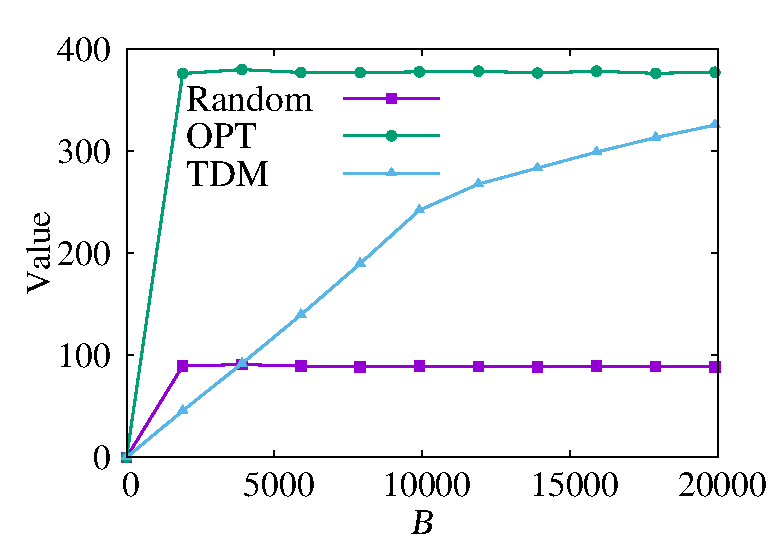
\includegraphics[width=0.7\textwidth]{BudgetChangeV.eps}
    \label{fig:gender_trend}
    \end{minipage}
  }

  \subfigure[The number of participants]{
  \centering
  \begin{minipage}[b]{0.5\textwidth}
  	\centering
    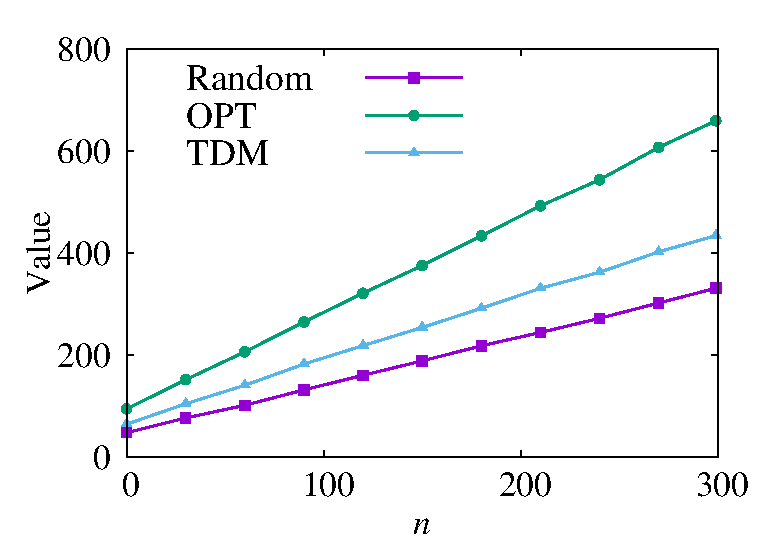
\includegraphics[width=0.7\textwidth]{AgentChangeV.eps}
    \label{fig:education_trend}
    \end{minipage}
  }
  \vspace{-0.2cm}
  \caption{Impact of varying the budget and the number of participants}
  \vspace{-0.2cm}
\end{figure}
In Fig. $2(a)$, we show the total value contributed by selected participants with varying budget. The number of participants $n$ is set to be $200$. We vary the budget from $0$ to $20000$ with the increment of $2000$. The arrival time and departure time are uniformly distributed in $[1,T]$. The discounting function in our evaluation is set to $F(t) = 0.9^t$, so the time-discounting value of participant $i$ is $v_i(t) = 0.9^tv_i$. The value and cost of each participant are randomly selected. All the results are averaged over 200 rounds. We observe that as the budget increases, the total value is becoming higher before the saturation is achieved. We note that when the budget is small, the value of TDM is less than value gained by random selection scheme. This is because that several participants will lose the auction with the small budget. These participants will be selected later or never. Due to the time-discounting property of values, the total value will decrease dramatically with time. However, we note that even with the strong constraint of truthfulness, our mechanism still achieves superior performance to the random scheme.

In Fig. $2(b)$, we vary the number of participants $n$ from $0$ to $600$ and fix the budget to $15000$. We can observe that with more participants, the total value increases. This is due to the fact that with more participants, the probability of the appearance of participants with high efficiencies gets higher.

\begin{figure}[!t]
  \centering
  \subfigure[Different budgets]{
  \begin{minipage}[b]{0.5\textwidth}
  	\centering
    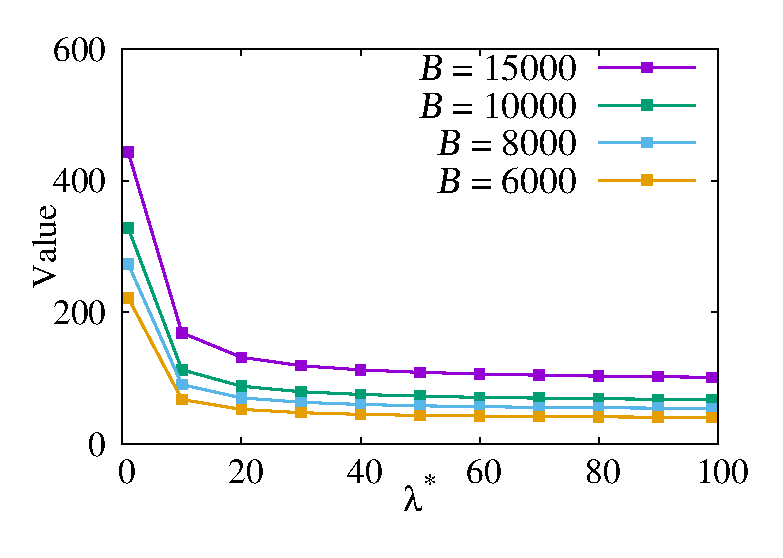
\includegraphics[width=0.7\textwidth]{BudgetLambda.eps}
    \label{fig:gender_trend}
    \end{minipage}
  }
  \subfigure[Different numbers of participants]{
  \begin{minipage}[b]{0.5\textwidth}
  \centering
    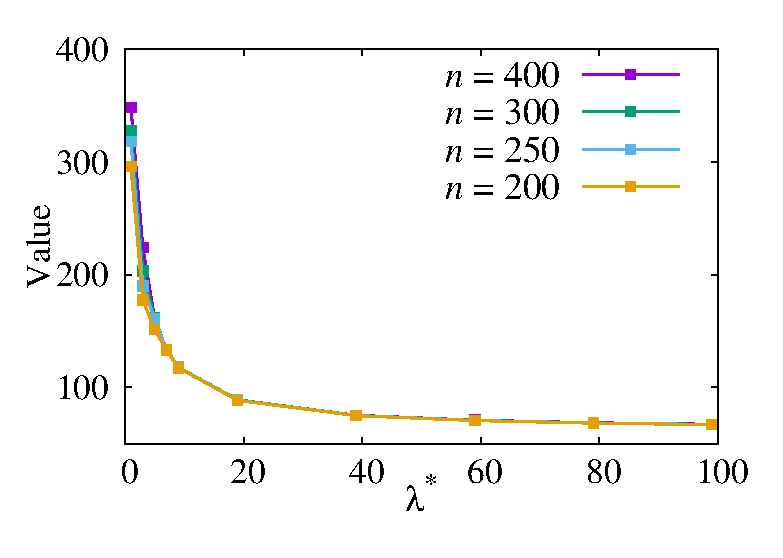
\includegraphics[width=0.7\textwidth]{AgentLambda.eps}
    \label{fig:education_trend}
    \end{minipage}
  }
  \vspace{-0.2cm}
  \caption{Impact of $\lambda\ (\lambda=\lambda_{min}+\frac{\lambda^*}{100}(\lambda_{max}-\lambda_{min}))$.}
  \vspace{-0.2cm}
\end{figure}
We then find the effect of the system parameter $\lambda$ on the total value, with different budget and number of participants.

In Fig. $3(a)$ and Fig. $3(b)$, we intend to investigate the effect of the system parameter $\lambda$. According to inequality $(9)$, $\lambda$ has an upper bound $\lambda_{max}= \frac{1}{\epsilon}\left(\frac{U}{L}\right)^{l-2}$ and a lower bound $\lambda_{min}=2\left(\frac{U}{L}\right)^{l-1}$, but we don't know how to choose $\lambda$ to maximize the value (even though we can  guarantee a constant competitive ratio). We divide the interval $[\lambda_{min}, \lambda_{max})$ into 100 pieces. We should also consider the effect of different budgets and participants. These two figures show us that with  $\lambda$ getting closer to $\lambda_{min}$, the value is getting higher regardless of the different budgets and participant numbers. This is because when $\lambda$ gets smaller, the threshold gets larger and the total value increases as well. The premise of this phenomenon is the huge number of participants. Considering that there are rare participants competing in this auction, if the threshold is large, some participants will be selected later. The total value will decrease due to the time-discounting property. When there are plentiful participants, the participants with less efficiency will lose and never be selected. In addition, we can also see the competitive ratio in expression $(8)$ has a negative correlation with $\lambda$.
%% The file named.bst is a bibliography style file for BibTeX 0.99c
\subsection{Select Ratio}
In Fig.4(a) and Fig.4(b), we intend to investigate the selected ratio with various numbers of participants and budget respectively. We first vary the budget from 6000 to 15000, with different numbers of participants. As shown in Fig.4(a), the selected ratio increases when the budget gets higher. We can also see that with a fixed budget, the selected ratio decrease with the number of participants. It may be because of the marginal effect. In Fig.4(b), the marginal effect is shown more significant. We infer that when the number of participants gets larger, the budget may be not enough to pay for them. 
\begin{figure}[!t]
  \centering
  \subfigure[Different budgets]{
  \begin{minipage}[b]{0.5\textwidth}
  	\centering
    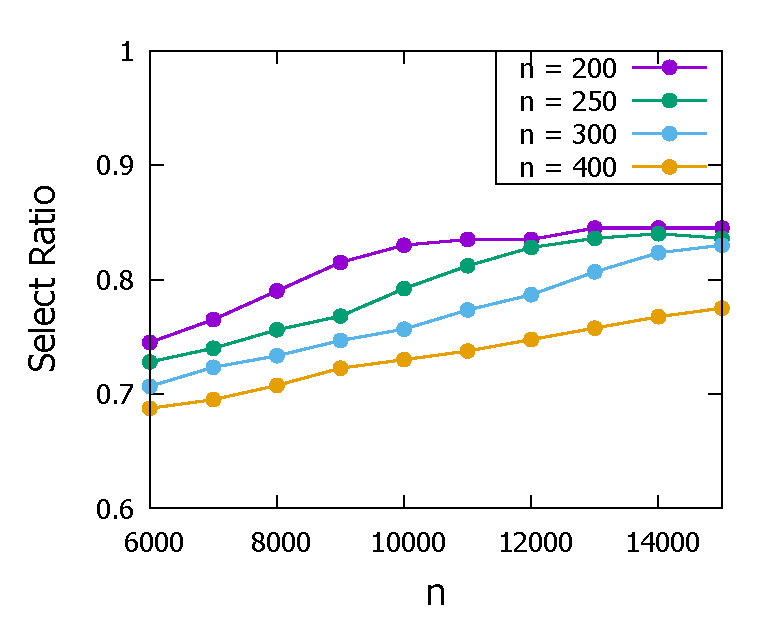
\includegraphics[width=0.7\textwidth]{RatioBudget.eps}
    \label{fig:gender_trend}
    \end{minipage}
  }
  \subfigure[Different numbers of participants]{
  \begin{minipage}[b]{0.5\textwidth}
  \centering
    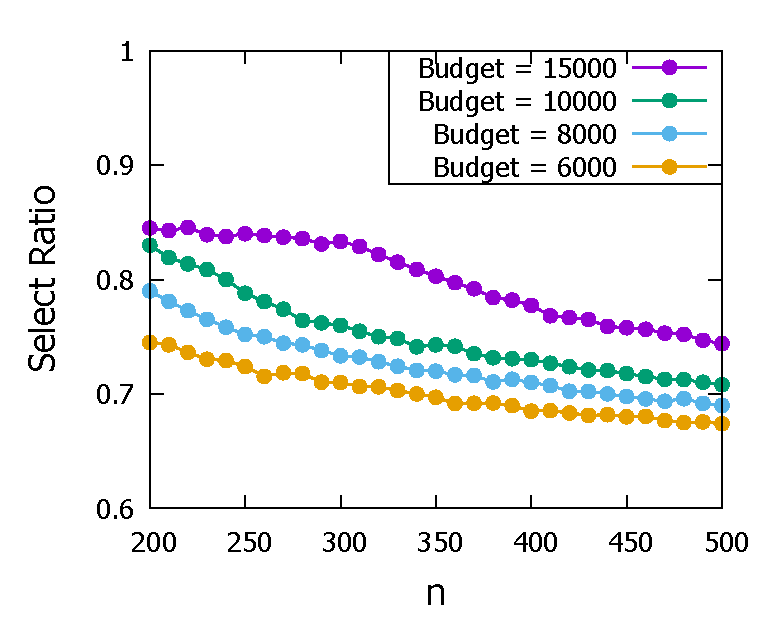
\includegraphics[width=0.7\textwidth]{AgentRatio.eps}
    \label{fig:education_trend}
    \end{minipage}
  }
  \vspace{-0.2cm}
  \caption{Select Ratio}
  \vspace{-0.2cm}
\end{figure}
\subsection{Budget Utilization}
We also intend to find the utilization of budget in our experiment. With the similar setup, the number of participants is varying from 200 to 800 and the budget is varying from 6000 to 15000. In Fig.5(a), it is shown that for a fixed number of participants, the utilization of budget is decreasing with more budget. And with a fixed budget, the utilization increases with the number of participants, which is commonsensible. In Fig.5(b), the marginal effect of utilization of budget is evident. It inspire that for an crowdsensing application with fixed registered participants, adding more budget may not bring more utility for the reason of marginal effect. This result is consistent with the result found in Fig.2(a).
\begin{figure}[!t]
  \centering
  \subfigure[Different budgets]{
  \begin{minipage}[b]{0.5\textwidth}
  	\centering
    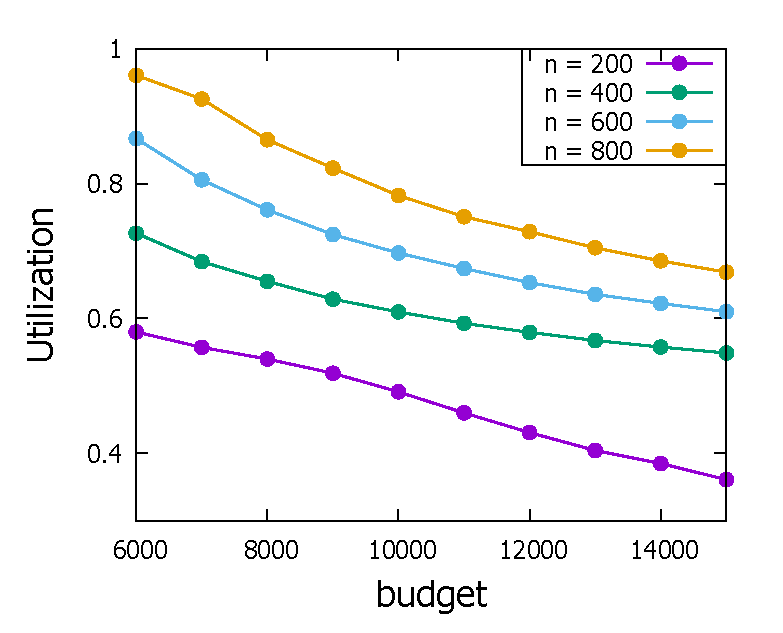
\includegraphics[width=0.7\textwidth]{UtiBudget.eps}
    \label{fig:gender_trend}
    \end{minipage}
  }
  \subfigure[Different numbers of participants]{
  \begin{minipage}[b]{0.5\textwidth}
  \centering
    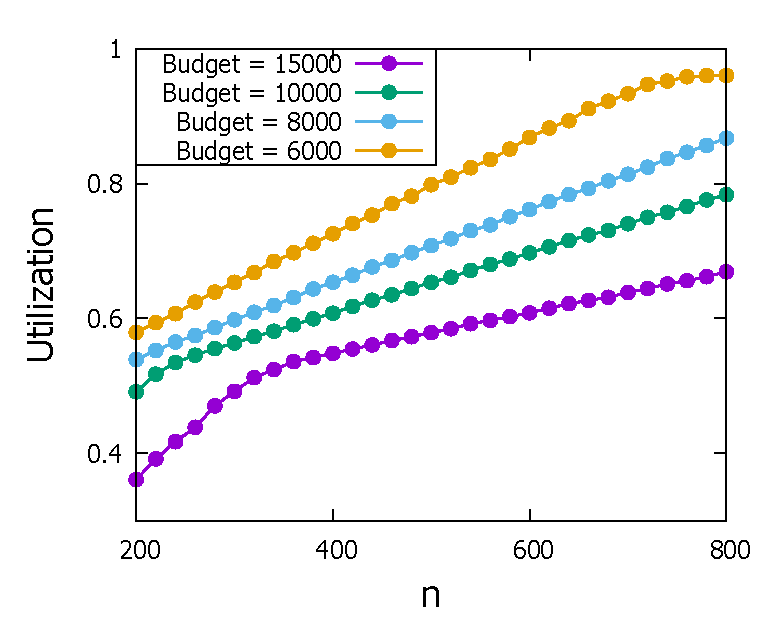
\includegraphics[width=0.7\textwidth]{AgentUti.eps}
    \label{fig:education_trend}
    \end{minipage}
  }
  \vspace{-0.2cm}
  \caption{Budget Utilization}
  \vspace{-0.2cm}
\end{figure}



\section{Conclusions And Future Work}
In this paper, we propose a strategy-proof and budget feasible online incentive mechanism for crowdsensing that considers the property of time-discounting values. The method proposed in our paper calculates a selection threshold, selects participants online and pays each selected participant with a carefully designed payment to guarantee strategy-proofness. We consider both the case with the function is a summation and a modular function. We have proved that no participant can get higher utility by misreporting her type. The competitive ratio of our mechanism is constant. The simulation results have shown that our mechanism achieves great performance in terms of the total obtained value.

In our paper, the time-discounting factor is $\beta_{-t}$,which is also used in the previous work. But in a general model, the value can be represented as $max(v_iF_i(t)+D_i(t),0)$, where $F_i$ and $D_i$ my be arbitrary functions. An attractive direction of fucture work is designing a general mechanism for the general discounting functions.
\bibliographystyle{abbrv}
\bibliography{paper}

\end{document}
